\documentclass[12pt,a4paper]{article}

% ─── Paquetes ───
\usepackage[utf8]{inputenc}
\usepackage[T1]{fontenc}
\usepackage{babel}
\babelprovide[import]{spanish}
\usepackage{geometry}
\usepackage{amsmath}
\usepackage{graphicx}
\usepackage{booktabs}
\usepackage{hyperref}
\usepackage{fancyhdr}
\usepackage{setspace}
\usepackage{parskip}
\usepackage{titlesec}
\usepackage{xcolor}
\usepackage{caption}

% ─── Configuración de página ───
\geometry{top=2.5cm, bottom=2.5cm, left=3cm, right=2.5cm}
\setlength{\parskip}{6pt}
\setlength{\headheight}{14pt}
\onehalfspacing

% ─── Encabezado / pie de página ───
\pagestyle{fancy}
\fancyhf{}
\fancyhead[L]{\small \textit{Predicci\'on de Riesgo Crediticio mediante RNA}}
\fancyhead[R]{\small \thepage}
\renewcommand{\headrulewidth}{0.5pt}

% ─── Formato de títulos ───
\titleformat{\section}{\large\bfseries}{\thesection.}{1em}{}
\titleformat{\subsection}{\normalsize\bfseries}{\thesubsection.}{1em}{}
\titleformat{\subsubsection}{\normalsize\bfseries}{\thesubsubsection.}{1em}{}

% ─── Hipervínculos ───
\hypersetup{
    colorlinks=true,
    linkcolor=black,
    citecolor=blue,
    urlcolor=blue
}

% ─── Información del documento ───
\title{\textbf{Predicci\'on de Riesgo Crediticio mediante Redes Neuronales Profundas: \\ Un Enfoque Anal\'itico para la Toma de Decisiones Financieras}}
\author{Sebastian Pabon Nunez \\ Jhofred Jahat Camacho Gomez}
\date{Junio 2026}

\begin{document}

% ═══════════════════════════════════════════════
% PORTADA
% ═══════════════════════════════════════════════
\begin{titlepage}
    \centering
    \vspace*{3cm}

    {\LARGE\textbf{UNIVERSIDAD NACIONAL DE MEDELLÍN}}\\[1.5cm]

    \rule{\textwidth}{0.5pt}\\[0.8cm]
    {\Large\textbf{Curso:}} Redes Neuronales y Algoritmos Bioinspirados\\[0.5cm]
    {\Large\textbf{Título del Proyecto:}} Sistema de Predicción de Riesgo Crediticio basado en Redes Neuronales Profundas\\[0.5cm]
    \rule{\textwidth}{0.5pt}\\[1.5cm]

    {\Large\textbf{Integrantes:}}\\[0.3cm]
    {\large Sebastian Pabon Nunez\\[0.1cm] Jhofred Jahat Camacho Gomez}\\[1.5cm]

    {\Large\textbf{Docente:}} Juan David Ospina Arango\\[0.5cm]
    {\Large\textbf{Fecha de Entrega:}} Junio 2026

    \vfill
\end{titlepage}

% ═══════════════════════════════════════════════
% 1. INTRODUCCIÓN
% ═══════════════════════════════════════════════
\section{Introducción}

El riesgo crediticio constituye una de las preocupaciones más críticas para las instituciones financieras en todo el mundo. En términos simples, se refiere a la probabilidad de que un prestatario incumpla con sus obligaciones de pago, lo que puede generar pérdidas económicas significativas para quienes otorgan el crédito (Basel Committee on Banking Supervision [BCBS], 2019). Esta problemática no solo afecta la estabilidad financiera de bancos y entidades de crédito, sino que también tiene repercusiones en la economía en general, ya que una gestión inadecuada del riesgo puede limitar el acceso al crédito para consumidores y empresas.

Las consecuencias de una evaluación deficiente del riesgo crediticio son múltiples. Desde una perspectiva financiera, los incumplimientos generan pérdidas directas que deben ser absorbidas por las instituciones, lo que reduce su rentabilidad y capacidad de otorgar nuevos préstamos. Desde un punto de vista macroeconómico, cuando múltiples entidades enfrentan niveles elevados de morosidad simultáneamente, puede desencadenarse una contracción del crédito que afecta el crecimiento económico (Mishkin, 2019). Por esta razón, los reguladores financieros exigen que las instituciones cuenten con sistemas robustos para evaluar y monitorear el riesgo de sus carteras de crédito.

Tradicionalmente, la evaluación crediticia se ha basado en criterios subjetivos y en el juicio de analistas que revisan manualmente las solicitudes de préstamo. Sin embargo, este enfoque presenta limitaciones significativas: es lento, costoso y propenso a inconsistencias. En las últimas décadas, la analítica de datos y el aprendizaje automático han transformado esta área, permitiendo que las instituciones financieras utilicen modelos predictivos para estimar de manera más precisa la probabilidad de incumplimiento (Lessmann et al., 2015).

Los modelos de \textit{credit scoring} ---también conocidos como modelos de puntuación crediticia--- analizan información histórica de miles o millones de préstamos para identificar patrones que distinguen a los clientes que cumplen con sus pagos de aquellos que incumplen. Estos modelos consideran múltiples factores como ingresos, nivel de endeudamiento, historial crediticio, características del préstamo y variables demográficas, entre otros. El resultado es una puntuación o probabilidad que refleja el riesgo asociado a cada solicitud (Thomas, 2009).

El presente proyecto aborda el problema de la predicción de riesgo crediticio mediante el desarrollo de un sistema basado en Redes Neuronales Artificiales (RNA), una técnica de aprendizaje profundo que ha demostrado capacidad para capturar relaciones complejas y no lineales entre variables. A diferencia de los métodos estadísticos tradicionales, las RNA pueden modelar interacciones sofisticadas entre múltiples factores simultáneamente, lo que las hace particularmente adecuadas para problemas donde las relaciones entre variables no siguen patrones simples (Goodfellow et al., 2016).

Más allá del aspecto técnico, este proyecto busca demostrar cómo la inteligencia artificial puede aportar valor tangible al sector financiero, mejorando la precisión de las evaluaciones de riesgo, reduciendo la subjetividad en la toma de decisiones y, en última instancia, contribuyendo a una gestión más eficiente del crédito. El sistema desarrollado no solo genera predicciones, sino que también ofrece explicaciones sobre los factores que más influyen en cada caso, lo que facilita la interpretación por parte de los analistas y fortalece la transparencia del proceso.

% ═══════════════════════════════════════════════
% 2. MARCO TEÓRICO
% ═══════════════════════════════════════════════
\section{Marco Teórico}

\subsection{El Credit Scoring: Concepto y Propósito}

El \textit{credit scoring} es un método estadístico utilizado para evaluar el riesgo de crédito de un solicitante. Su propósito es asignar una puntuación numérica que refleje la probabilidad de que una persona incumpla con sus obligaciones de pago dentro de un período determinado. Esta puntuación se calcula a partir de información histórica sobre el comportamiento crediticio del individuo, así como de características personales y financieras relevantes (Thomas, 2009).

Desde una perspectiva práctica, el credit scoring funciona como un sistema de clasificación: toma los datos de un solicitante y los asigna a una de dos categorías ---bajo riesgo o alto riesgo---. Las instituciones financieras utilizan esta clasificación para decidir si aprueban o rechazan una solicitud de préstamo, qué tasa de interés ofrecer, y cuál debe ser el monto máximo a otorgar. Un score alto indica baja probabilidad de incumplimiento, mientras que un score bajo sugiere mayor riesgo (Lessmann et al., 2015).

La importancia del credit scoring radica en que permite estandarizar el proceso de evaluación, reducir la subjetividad y acelerar la toma de decisiones. Además, al basarse en datos históricos, estos sistemas pueden identificar patrones que no serían evidentes para un analista humano, mejorando así la precisión de las predicciones.

\subsection{Predicción de Incumplimiento: El Problema del Default}

En el contexto crediticio, el término \textit{default} o incumplimiento se refiere a la situación en la que un prestatario no cumple con sus obligaciones de pago según los términos acordados. Esto puede manifestarse de diversas formas: pagos atrasados, falta total de pago, o la necesidad de reestructurar la deuda. Para las instituciones financieras, el default representa una pérdida económica directa, ya que el dinero prestado no se recupera en su totalidad (Basel Committee on Banking Supervision [BCBS], 2019).

Predecir el default es, en esencia, un problema de clasificación binaria. El modelo debe analizar las características de un préstamo o solicitante y determinar si es más probable que el crédito se clasifique como ``cumplido'' (clase 0) o como ``incumplido'' (clase 1). La dificultad del problema radica en que las relaciones entre las variables no siempre son lineales ni evidentes. Por ejemplo, un alto nivel de ingresos no necesariamente garantiza el cumplimiento si el solicitante tiene un nivel de endeudamiento excesivo o un historial de pagos irregulares (Mishkin, 2019).

Los modelos predictivos abordan este problema identificando patrones en datos históricos. Al analizar miles o millones de casos anteriores ---tanto de clientes que cumplieron como de aquellos que incumplieron---, el modelo aprende a reconocer las combinaciones de características que están asociadas con mayor probabilidad de incumplimiento. Esta información se utiliza luego para evaluar nuevos casos y estimar su nivel de riesgo (Thomas, 2009).

\subsection{Modelos Predictivos en la Evaluación Crediticia}

Los modelos predictivos han revolucionado la evaluación crediticia al permitir que las instituciones financieras tomen decisiones más informadas y objetivas. Estos modelos utilizan técnicas estadísticas y de aprendizaje automático para analizar grandes volúmenes de datos y generar predicciones sobre el comportamiento futuro de los prestatarios (Lessmann et al., 2015).

Entre las técnicas más utilizadas se encuentran la regresión logística, los árboles de decisión, los modelos de bosques aleatorios y, más recientemente, las redes neuronales. Cada una de estas técnicas tiene sus fortalezas y limitaciones. La regresión logística, por ejemplo, es ampliamente utilizada por su simplicidad e interpretabilidad, pero puede tener dificultades para capturar relaciones no lineales complejas. Los árboles de decisión son más flexibles, pero pueden ser propensos al sobreajuste si no se controlan adecuadamente (Goodfellow et al., 2016).

Los modelos predictivos no solo mejoran la precisión de las evaluaciones, sino que también permiten a las instituciones financieras optimizar sus procesos, reducir costos operativos y gestionar mejor el riesgo de sus carteras. Además, al contar con estimaciones más precisas del riesgo, las instituciones pueden ofrecer tasas de interés más justas, premiando a los clientes de bajo riesgo y protegiéndose adecuadamente contra aquellos con mayor probabilidad de incumplimiento (Mishkin, 2019).

\subsection{Redes Neuronales Artificiales: Una Aproximación al Aprendizaje Profundo}

Las Redes Neuronales Artificiales (RNA) son modelos computacionales inspirados en la estructura y funcionamiento del cerebro humano. Están compuestas por unidades de procesamiento llamadas neuronas artificiales, que se organizan en capas interconectadas. Cada neurona recibe entradas, las procesa mediante una función de activación, y produce una salida que se transmite a las neuronas de la siguiente capa (Goodfellow et al., 2016).

Lo que distingue a las RNA de otros modelos predictivos es su capacidad para aprender representaciones complejas de los datos. A medida que la información avanza a través de las capas de la red, se van extrayendo características de nivel creciente de abstracción. Esto permite que el modelo capture relaciones no lineales e interacciones sofisticadas entre las variables, algo que resulta particularmente valioso en problemas como la predicción de riesgo crediticio, donde múltiples factores interactúan de maneras complejas (LeCun et al., 2015).

El término ``aprendizaje profundo'' (\textit{deep learning}) se refiere al uso de redes neuronales con múltiples capas ocultas. Estas arquitecturas profundas han demostrado ser excepcionalmente efectivas en una amplia variedad de tareas, desde el reconocimiento de imágenes hasta el procesamiento del lenguaje natural. En el contexto financiero, las RNA han mostrado capacidad para superar a los métodos tradicionales en tareas de predicción de riesgo, especialmente cuando se dispone de grandes volúmenes de datos y de poder computacional suficiente para entrenar modelos complejos (Goodfellow et al., 2016).

Es importante destacar que, aunque las RNA pueden ser más difíciles de interpretar que modelos más simples como la regresión logística, existen técnicas ---como SHAP (Shapley Additive Explanations)--- que permiten explicar las predicciones individuales y comprender qué factores influyeron más en cada caso. Esto hace que las RNA no solo sean poderosas en términos predictivos, sino también útiles para la toma de decisiones informadas (Lundberg \& Lee, 2017).

% ═══════════════════════════════════════════════
% 3. METODOLOGÍA
% ═══════════════════════════════════════════════
\section{Metodología}

El desarrollo del sistema de predicción de riesgo crediticio siguió una metodología estructurada que abarcó desde la preparación de los datos hasta la evaluación del modelo final. Cada etapa del proceso fue diseñada para garantizar la calidad de los resultados y la robustez del sistema.

\subsection{Preparación de los Datos}

El punto de partida del proyecto fue el conjunto de datos \textit{LendingClub Loan Data}, que contiene información sobre préstamos otorgados a través de la plataforma LendingClub entre 2007 y 2015. Este dataset incluye 887,379 registros con 74 variables diferentes, abarcando información demográfica, financiera y crediticia de los solicitantes, así como detalles sobre los préstamos y su estado final.

La primera tarea consistió en comprender la estructura de los datos y definir la variable objetivo. En este caso, la variable a predecir es \texttt{loan\_status}, que indica si un préstamo fue cumplido (\textit{Fully Paid}) o incumplido (\textit{Charged Off}, \textit{Default}, o \textit{Late}). Dado que el dataset original contiene múltiples categorías intermedias y estados ambiguos ---como \textit{Current}, \textit{In Grace Period}, o \textit{Late (16--30 days)}---, fue necesario realizar una recodificación cuidadosa para convertir el problema en una clasificación binaria clara: clase 0 para préstamos cumplidos y clase 1 para préstamos incumplidos. Los registros con estados ambiguos fueron excluidos del análisis para evitar ambigüedades en el entrenamiento del modelo.

Tras esta recodificación, el dataset quedó conformado por aproximadamente 190,000 registros, con una distribución de clases que refleja un desbalance moderado: alrededor del 77\% de los préstamos fueron cumplidos y el 23\% incumplidos. Esta proporción es consistente con las tasas de morosidad observadas en el sector financiero y justifica el uso de estrategias específicas para manejar el desbalance durante el entrenamiento (Lessmann et al., 2015).

\subsection{Limpieza y Transformación de Datos}

Una vez definida la variable objetivo, se procedió a la limpieza y transformación de las variables predictoras. Este proceso es fundamental, ya que la calidad de los datos tiene un impacto directo en el desempeño del modelo. Los datos crudos suelen contener valores faltantes, variables redundantes, y características que no aportan información relevante para la predicción.

El primer paso fue identificar y eliminar las columnas con un porcentaje elevado de valores faltantes. Específicamente, se excluyeron aquellas variables que presentaban más del 10\% de valores nulos, ya que la imputación de grandes cantidades de datos faltantes puede introducir sesgos y reducir la confiabilidad del modelo. Entre las variables eliminadas se encuentran \texttt{mths\_since\_last\_delinq}, \texttt{mths\_since\_last\_major\_derog}, y diversas variables relacionadas con crédito rotativo e información conjunta.

Posteriormente, se identificaron y eliminaron las variables altamente correlacionadas entre sí. Cuando dos variables están fuertemente correlacionadas (por ejemplo, con un coeficiente de correlación superior a 0.6), aportan información redundante al modelo, lo que puede causar problemas de multicolinealidad y dificultar el entrenamiento. Variables como \texttt{total\_rev\_hi\_lim}, \texttt{total\_acc}, \texttt{funded\_amnt}, y \texttt{total\_pymnt} fueron excluidas por presentar alta correlación con otras variables ya incluidas en el modelo.

También se eliminaron las variables con varianza cercana a cero, es decir, aquellas que prácticamente no varían entre los registros. Estas variables no aportan información discriminativa y solo añaden ruido al modelo. Ejemplos de variables eliminadas por esta razón incluyen \texttt{collections\_12\_mths\_ex\_med}, \texttt{policy\_code}, y \texttt{acc\_now\_delinq}.

Finalmente, se seleccionaron las variables más relevantes para el modelamiento. La selección final incluyó 10 variables clave: \texttt{last\_pymnt\_amnt} (último pago recibido), \texttt{recoveries} (recuperaciones post-incumplimiento), \texttt{out\_prncp} (capital pendiente), \texttt{int\_rate} (tasa de interés), \texttt{term} (plazo del préstamo), \texttt{total\_rec\_late\_fee} (total de cargos por mora), \texttt{tot\_cur\_bal} (saldo total actual), \texttt{dti} (relación deuda-ingresos), \texttt{initial\_list\_status} (estatus inicial en lista), y \texttt{loan\_amnt} (monto del préstamo). Es importante señalar que varias de estas variables reflejan información posterior al desembolso del préstamo, lo que significa que el modelo es más adecuado para tareas de monitoreo de cartera y cobranza temprana que para la evaluación de solicitudes iniciales.

\subsection{Construcción del Pipeline de Preprocesamiento}

Antes de entrenar el modelo, fue necesario construir un pipeline de preprocesamiento que transformara los datos crudos en un formato adecuado para la red neuronal. Este pipeline incluye varios pasos secuenciales.

Para las variables numéricas, se aplicó una imputación por mediana para manejar cualquier valor faltante restante, seguida de un escalamiento con \texttt{StandardScaler}. El escalamiento es esencial para las redes neuronales, ya que asegura que todas las variables tengan una escala similar, lo que facilita el entrenamiento y mejora la convergencia del modelo.

Para las variables categóricas, se utilizó una codificación ordinal que convierte las categorías en valores numéricos. Esto permite que la red neuronal procese este tipo de variables sin perder información.

El pipeline se implementó utilizando \texttt{ColumnTransformer} de scikit-learn, lo que garantiza que las transformaciones se apliquen de manera consistente tanto durante el entrenamiento como durante la predicción de nuevos casos. Esta consistencia es crucial para evitar errores y asegurar que el modelo funcione correctamente en producción.

\subsection{Entrenamiento del Modelo}

El entrenamiento del modelo siguió un enfoque riguroso que incluyó la división de los datos en conjuntos de entrenamiento, validación y prueba, así como la optimización de hiperparámetros mediante búsqueda aleatoria.

Los datos se dividieron de manera estratificada para mantener la proporción original de clases en cada subconjunto: 60\% para entrenamiento, 20\% para validación y 20\% para prueba. La división estratificada es importante cuando se trabaja con clases desbalanceadas, ya que asegura que cada subconjunto sea representativo de la distribución original.

Para el entrenamiento de la red neuronal, se utilizó una estrategia de ponderación de clases que asigna mayor peso a la clase minoritaria (incumplimiento) durante el entrenamiento. Esto obliga al modelo a prestar más atención a los casos de incumplimiento, mejorando su capacidad para detectarlos. La ponderación se calculó automáticamente utilizando la función \texttt{compute\_class\_weight} de scikit-learn con la opción \texttt{balanced}.

La arquitectura de la red neuronal fue optimizada mediante una búsqueda aleatoria de hiperparámetros que evaluó 25 configuraciones diferentes. El espacio de búsqueda incluyó variaciones en el número de capas ocultas (2 a 5), el número de neuronas por capa (64 a 384), la tasa de aprendizaje (0.0001 a 0.002), el tipo y fuerza de regularización (L1, L2, L1\_L2, o ninguna), la tasa de dropout (0.1 a 0.5), y la inclusión o no de normalización por lotes.

La mejor configuración encontrada fue la siguiente: 3 capas ocultas con 384, 230 y 138 neuronas respectivamente, regularización L1 con intensidad 1e-05, tasa de aprendizaje de 0.002, dropout de 0.5, normalización por lotes activada, y un factor de reducción de 0.6 para el tamaño de las capas sucesivas. Esta arquitectura permite que el modelo capture relaciones complejas mientras se protege contra el sobreajuste mediante la regularización y el dropout.

El modelo fue entrenado utilizando el optimizador Adam, que es ampliamente reconocido por su eficiencia y capacidad de convergencia. La función de pérdida utilizada fue \textit{Binary Cross-Entropy} con suavizado de etiquetas (\textit{label smoothing}) de 0.03. Este valor fue seleccionado mediante búsqueda aleatoria dentro del espacio \{0.0, 0.01, 0.03, 0.05\}, y tiene como propósito evitar que el modelo genere predicciones excesivamente confiadas (cercanas a 0 o 1), lo cual mejora la generalización y reduce el sobreajuste a las etiquetas de entrenamiento (Szegedy et al., 2016). Durante el entrenamiento, se implementaron mecanismos de detención temprana y reducción de la tasa de aprendizaje para evitar el sobreajuste y asegurar la convergencia óptima.

Un aspecto importante del entrenamiento fue el ajuste del umbral de decisión. Por defecto, los modelos de clasificación utilizan un umbral de 0.5 para decidir si una predicción se clasifica como clase 0 o clase 1. Sin embargo, en el contexto de riesgo crediticio, puede ser más importante detectar la mayor cantidad posible de casos de incumplimiento, incluso si esto implica aceptar más falsos positivos. Por esta razón, el umbral se optimizó maximizando el F2-score, una métrica que pondera más el recall (sensibilidad) que la precisión. El umbral óptimo encontrado fue de 0.54933, lo que refleja una política de detección sensible orientada a identificar la mayor cantidad posible de casos riesgosos.

Para garantizar la reproducibilidad de los resultados, se fijó una semilla aleatoria global de 42, aplicada consistentemente en la división de datos, la inicialización de pesos del modelo, la búsqueda de hiperparámetros y todos los componentes estocásticos del pipeline. El modelo fue implementado utilizando TensorFlow 2.21.0 con Keras, y el entrenamiento se ejecutó en un entorno Google Colab con acelerador GPU T4. La semilla también se propagó a las variables de entorno (\texttt{PYTHONHASHSEED}), a los módulos \texttt{random} y \texttt{numpy}, y al generador de TensorFlow mediante \texttt{tf.random.set\_seed}.

\subsection{Criterios de Evaluación}

La evaluación del modelo se realizó comparando su desempeño contra una línea base de regresión logística, utilizando métricas tales como PR-AUC, ROC-AUC, precisión, recall y F1-score. Los resultados detallados de esta comparación se presentan en la Sección~\ref{sec:resultados}.

% ═══════════════════════════════════════════════
% 4. ANÁLISIS EXPLORATORIO DE DATOS (EDA)
% ═══════════════════════════════════════════════
\section{Análisis Exploratorio de Datos (EDA)}

El análisis exploratorio de datos (EDA, por sus siglas en inglés) es una etapa fundamental en cualquier proyecto de ciencia de datos. Su propósito es comprender la estructura de los datos, identificar patrones, detectar anomalías, y formular hipótesis antes de proceder con el modelamiento predictivo. En el contexto de este proyecto, el EDA permitió descubrir qué variables están más relacionadas con el riesgo de incumplimiento y cómo se comportan las relaciones entre ellas.

Más allá de ser un paso técnico, el EDA es una oportunidad para contar una historia con los datos. Cada gráfico, cada correlación, y cada estadística descriptiva aporta información valiosa sobre el comportamiento de los prestatarios y los factores que influyen en su capacidad para cumplir con las obligaciones de pago. A continuación, se presentan los hallazgos más relevantes del análisis exploratorio, organizados de manera narrativa para facilitar su comprensión e interpretación.

\subsection{Comprensión de las Relaciones entre Variables: Correlación de Pearson}

El primer paso del análisis exploratorio fue examinar las relaciones lineales entre las variables numéricas mediante la matriz de correlación de Pearson. Esta matriz es una herramienta estadística que mide el grado de asociación lineal entre pares de variables. Los valores de correlación oscilan entre \(-1\) y \(1\): un valor cercano a 1 indica una correlación positiva fuerte (cuando una variable aumenta, la otra también), un valor cercano a \(-1\) indica una correlación negativa fuerte (cuando una variable aumenta, la otra disminuye), y un valor cercano a 0 indica que no hay una relación lineal significativa entre las variables.

\begin{figure}[htbp]
    \centering
    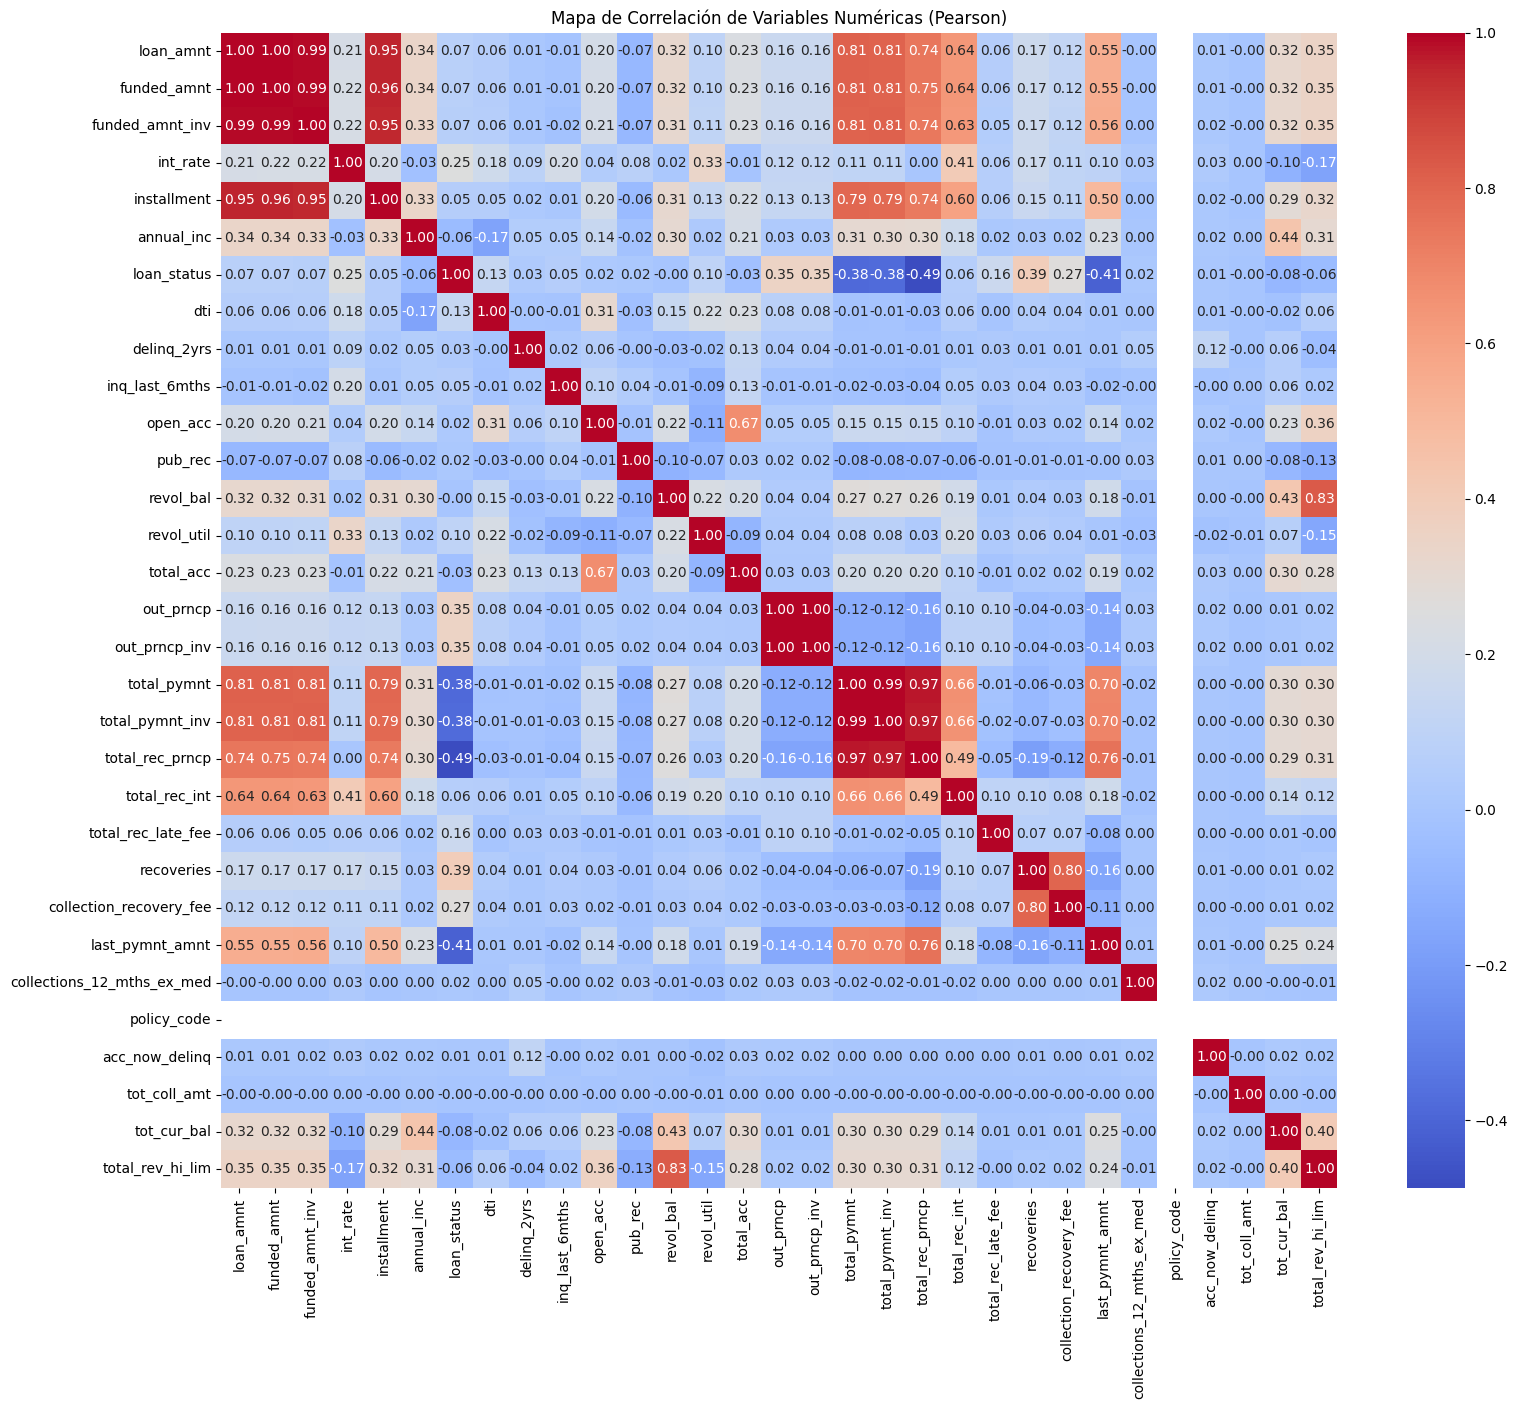
\includegraphics[width=0.85\textwidth]{./images/pearson_correlacion1.png}
    \caption{Matriz de Correlación de Variables Numéricas (Pearson)}
    \label{fig:pearson}
\end{figure}

\textit{Nota.} Mapa de calor que muestra los coeficientes de correlación de Pearson entre todas las variables numéricas del dataset. Los valores cercanos a 1 (en tonos rojos) indican correlaciones positivas fuertes, mientras que los valores cercanos a \(-1\) (en tonos azules) indican correlaciones negativas fuertes. Los valores cercanos a 0 (en tonos blancos) sugieren ausencia de correlación lineal.

La observación de la matriz de correlación de Pearson revela varios patrones de alta relevancia. En primer lugar, se identifican tres grupos de variables con correlaciones extremadamente altas (superiores a 0.9), lo que indica una redundancia significativa en la información que aportan:

\textbf{Grupo 1 --- Monto del préstamo:} Las variables \texttt{loan\_amnt}, \texttt{funded\_amnt} y \texttt{funded\_amnt\_inv} presentan correlaciones prácticamente perfectas entre sí (\texttt{loan\_amnt} \(\leftrightarrow\) \texttt{funded\_amnt} = 1.00; \texttt{loan\_amnt} \(\leftrightarrow\) \texttt{funded\_amnt\_inv} = 0.99; \texttt{funded\_amnt} \(\leftrightarrow\) \texttt{funded\_amnt\_inv} = 0.99). Esto indica que las tres variables contienen esencialmente la misma información, por lo que incluir más de una de ellas en el modelo sería redundante.

\textbf{Grupo 2 --- Pagos totales:} Las variables \texttt{total\_pymnt}, \texttt{total\_pymnt\_inv} y \texttt{total\_rec\_prncp} también muestran correlaciones extremadamente altas (\texttt{total\_pymnt} \(\leftrightarrow\) \texttt{total\_pymnt\_inv} = 0.99; \texttt{total\_pymnt} \(\leftrightarrow\) \texttt{total\_rec\_prncp} = 0.97; \texttt{total\_pymnt\_inv} \(\leftrightarrow\) \texttt{total\_rec\_prncp} = 0.97). Esta fuerte redundancia sugiere que estas variables miden aspectos prácticamente idénticos del comportamiento de pago.

\textbf{Grupo 3 --- Capital pendiente:} Las variables \texttt{out\_prncp} y \texttt{out\_prncp\_inv} presentan una correlación perfecta de 1.00, lo que confirma que son versiones duplicadas de la misma información.

En segundo lugar, se observan correlaciones moderadas entre variables financieras clave y el estado del préstamo (\texttt{loan\_status}). Las variables más relacionadas con el estado del préstamo según Pearson son:

\begin{center}
\begin{tabular}{lr}
\toprule
Variable & Correlación Pearson \\
\midrule
total\_rec\_prncp & -0.49 \\
last\_pymnt\_amnt & -0.41 \\
total\_pymnt       & -0.38 \\
recoveries         &  0.39 \\
out\_prncp         &  0.35 \\
\bottomrule
\end{tabular}
\end{center}

Estos valores revelan patrones financieramente interpretables: un mayor total de pagos realizados (\texttt{total\_rec\_prncp}, \texttt{total\_pymnt}) y un último pago más alto (\texttt{last\_pymnt\_amnt}) se asocian negativamente con el incumplimiento, es decir, están relacionados con préstamos saludables. Por el contrario, mayores recuperaciones (\texttt{recoveries}) y un capital pendiente más elevado (\texttt{out\_prncp}) se asocian positivamente con estados de incumplimiento.

En tercer lugar, la tasa de interés (\texttt{int\_rate}) muestra una correlación positiva con variables asociadas al riesgo, como el plazo del préstamo y el monto solicitado. Esto tiene sentido desde una perspectiva financiera: los préstamos con mayor riesgo suelen tener tasas de interés más altas para compensar el mayor nivel de incertidumbre.

La relación deuda-ingresos (\texttt{dti}) también presenta correlaciones interesantes con otras variables financieras. Una DTI alta indica que una proporción significativa de los ingresos del prestatario se destina al pago de deudas, lo que puede ser un indicador de estrés financiero y mayor probabilidad de incumplimiento.

El hallazgo más importante de este análisis es la evidencia clara de multicolinealidad entre los grupos de variables identificados. Variables como \texttt{funded\_amnt}, \texttt{funded\_amnt\_inv} y \texttt{loan\_amnt}, o como \texttt{total\_pymnt}, \texttt{total\_pymnt\_inv} y \texttt{total\_rec\_prncp}, deberían evaluarse para eliminación o reducción dimensional, ya que su inclusión simultánea en un modelo puede causar inestabilidad en las estimaciones y dificultar la interpretación de los coeficientes. Esta constatación fundamenta la decisión metodológica de eliminar variables redundantes descrita en la sección de preparación de datos.

Sin embargo, la correlación de Pearson tiene una limitación importante: solo captura relaciones lineales. En la práctica, las relaciones entre variables financieras pueden ser más complejas y no lineales. Por esta razón, fue necesario complementar el análisis con una medida de correlación que pudiera capturar este tipo de relaciones.

\subsection{Más Allá de la Linealidad: Correlación de Spearman}

Para capturar relaciones no lineales entre las variables, se calculó la matriz de correlación de Spearman. A diferencia de la correlación de Pearson, que mide la asociación lineal, la correlación de Spearman evalúa la asociación monótona, es decir, la tendencia de una variable a aumentar o disminuir de manera consistente a medida que aumenta la otra, independientemente de si la relación es lineal o no.

\begin{figure}[htbp]
    \centering
    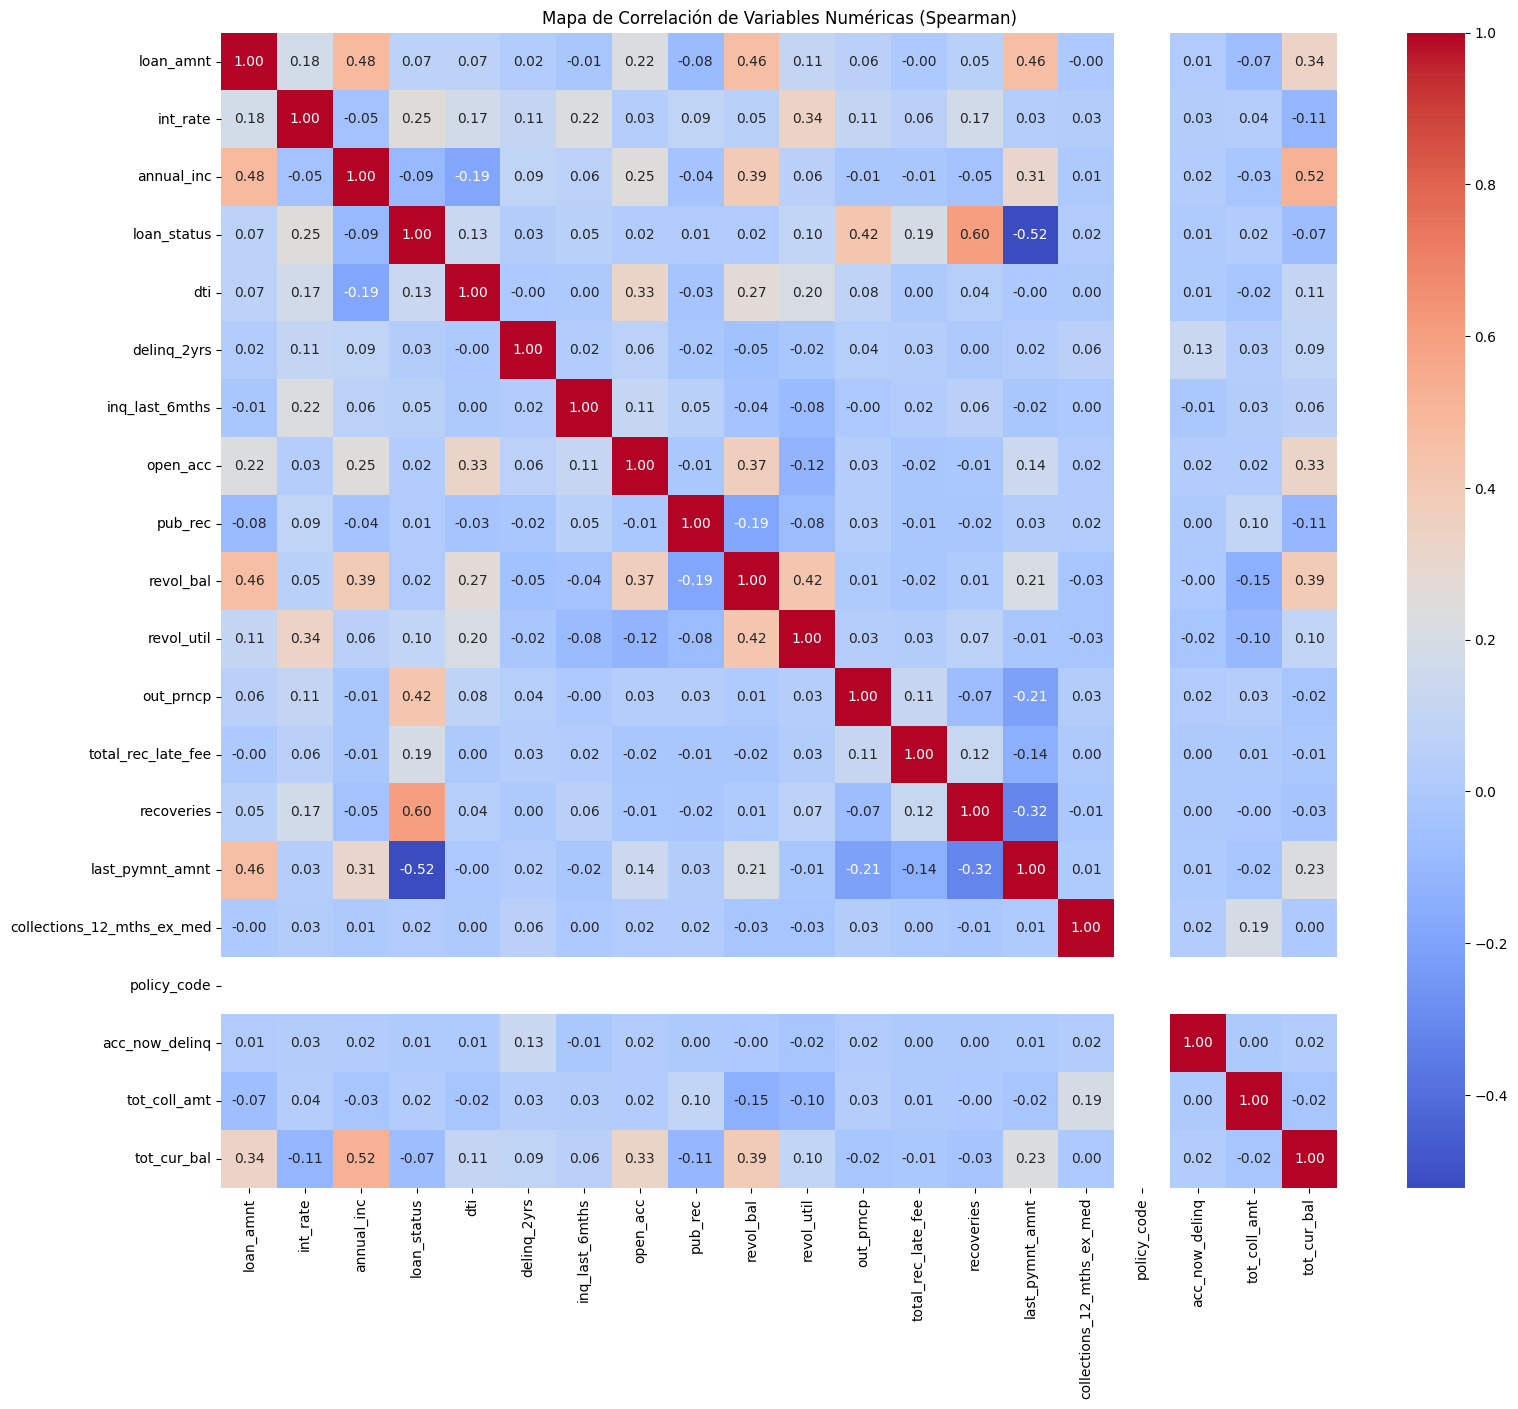
\includegraphics[width=0.85\textwidth]{./images/spearman.png}
    \caption{Matriz de Correlación de Variables Numéricas (Spearman)}
    \label{fig:spearman}
\end{figure}

\textit{Nota.} Mapa de calor que muestra los coeficientes de correlación de Spearman entre todas las variables numéricas del dataset. Esta medida captura relaciones monótonas, incluyendo aquellas que no son estrictamente lineales, proporcionando una visión más completa de las asociaciones entre variables.

El análisis de Spearman proporciona hallazgos de mayor profundidad que el análisis de Pearson, particularmente en lo que respecta a la relación entre las variables explicativas y el estado del préstamo. Las variables más relacionadas con \texttt{loan\_status} según el coeficiente de Spearman son:

\begin{center}
\begin{tabular}{lr}
\toprule
Variable & Correlación Spearman \\
\midrule
recoveries        &  0.60 \\
last\_pymnt\_amnt & -0.52 \\
out\_prncp        &  0.42 \\
int\_rate         &  0.25 \\
total\_rec\_late\_fee & 0.19 \\
\bottomrule
\end{tabular}
\end{center}

Estos valores revelan que \texttt{recoveries} (0.60) es la variable más asociada al estado del préstamo bajo esta medida, superando incluso a \texttt{last\_pymnt\_amnt} (-0.52). Cuando existen recuperaciones de deuda, estas suelen estar relacionadas con préstamos problemáticos o incumplidos, lo que convierte a esta variable en un indicador fuerte de deterioro crediticio. Por su parte, \texttt{last\_pymnt\_amnt} presenta una relación negativa fuerte: pagos finales altos suelen indicar préstamos saludables, mientras que pagos finales bajos se asocian a préstamos en mora o incumplimiento.

El capital pendiente (\texttt{out\_prncp}, 0.42) también muestra una asociación moderada-fuerte, indicando que saldos pendientes elevados están relacionados con estados de mayor riesgo. La tasa de interés (\texttt{int\_rate}, 0.25) y los cargos por mora (\texttt{total\_rec\_late\_fee}, 0.19) completan el grupo de variables con mayor poder discriminante.

En cuanto a las correlaciones entre variables explicativas, las más relevantes son:

\begin{center}
\begin{tabular}{lc}
\toprule
Variables & Correlación Spearman \\
\midrule
annual\_inc \(\leftrightarrow\) tot\_cur\_bal & 0.52 \\
loan\_amnt \(\leftrightarrow\) annual\_inc    & 0.48 \\
loan\_amnt \(\leftrightarrow\) revol\_bal    & 0.46 \\
loan\_amnt \(\leftrightarrow\) last\_pymnt\_amnt & 0.46 \\
revol\_bal \(\leftrightarrow\) revol\_util   & 0.42 \\
\bottomrule
\end{tabular}
\end{center}

Estas correlaciones revelan patrones financieramente interpretables: las personas con mayores ingresos tienden a tener mayores saldos totales; los préstamos más grandes suelen otorgarse a personas con ingresos más altos; y los usuarios con balances rotativos altos presentan mayor utilización del crédito.

Un hallazgo particularmente importante del análisis de Spearman es que no se observan correlaciones extremadamente altas (superiores a 0.8) entre las variables explicativas seleccionadas, lo que indica que no existe una multicolinealidad severa en el conjunto final de variables. Esto es positivo tanto para modelos lineales como para redes neuronales, ya que garantiza que cada variable aporta información relativamente independiente al modelo.

La comparación entre las matrices de Pearson y Spearman revela diferencias significativas. Mientras que Pearson mostraba correlaciones perfectas entre variables redundantes (como \texttt{loan\_amnt} \(\leftrightarrow\) \texttt{funded\_amnt} = 1.00), Spearman proporciona una visión más matizada de las asociaciones una vez eliminadas las variables redundantes. Además, Spearman captura con mayor fuerza la relación entre \texttt{recoveries} y \texttt{loan\_status} (0.60 frente a 0.39 de Pearson), lo que sugiere que esta relación tiene un componente no lineal que Pearson no logra capturar completamente.

El análisis de Spearman también revela asociaciones que no eran evidentes en el análisis de Pearson, como la relación entre ingresos anuales y saldo total corriente (0.52), lo que enriquece la comprensión del comportamiento de los datos y aporta información valiosa para la selección de variables.

\subsection{Identificación de Variables Clave: Análisis de Importancia}

Una vez comprendidas las relaciones entre variables, el siguiente paso fue identificar cuáles de ellas tienen mayor poder discriminante para predecir el riesgo de incumplimiento. Para ello, se entrenó un modelo de Random Forest ---un algoritmo de aprendizaje automático basado en árboles de decisión--- configurado con 50 estimadores, profundidad máxima de 10, semilla aleatoria de 42 y ejecución en paralelo (\texttt{n\_jobs=-1}), y se extrajo la importancia relativa de cada variable.

El Random Forest es una herramienta útil para este propósito porque puede capturar relaciones no lineales e interacciones entre variables, y proporciona una medida de importancia que refleja cuánto contribuye cada variable a la capacidad predictiva del modelo. Aunque esta medida es exploratoria y no constituye una explicación formal del modelo final de red neuronal, sí proporciona una guía valiosa sobre qué variables parecen concentrar el poder discriminante en el dataset.

\begin{figure}[htbp]
    \centering
    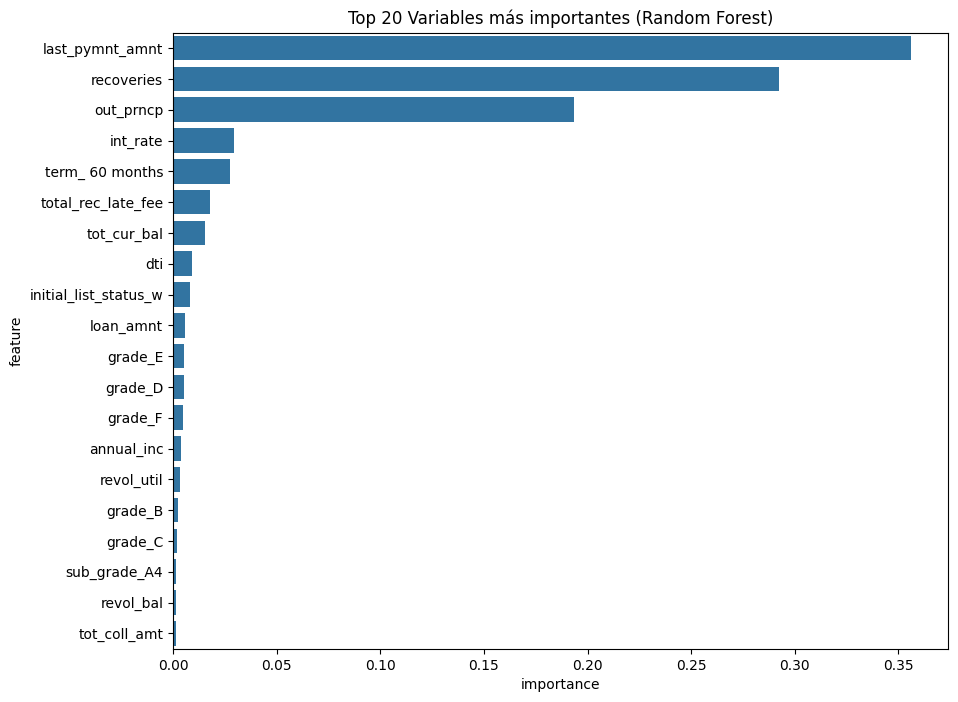
\includegraphics[width=0.85\textwidth]{./images/20var_mas_importantes_eda.png}
    \caption{Top 20 Variables más Importantes según Random Forest}
    \label{fig:importancia}
\end{figure}

\textit{Nota.} Gráfico de barras que muestra las 20 variables con mayor importancia según el modelo Random Forest. La importancia se calcula como la reducción promedio en la impureza de los nodos del árbol cuando se utiliza la variable para dividir los datos. Valores más altos indican mayor contribución a la capacidad predictiva del modelo.

Los resultados del análisis de importancia revelan una concentración notable del poder predictivo en un grupo reducido de variables. Las tres variables más importantes acumulan aproximadamente el 84\% de toda la importancia del modelo:

\begin{center}
\begin{tabular}{lr}
\toprule
Variable & Importancia \\
\midrule
last\_pymnt\_amnt & 0.36 \\
recoveries        & 0.29 \\
out\_prncp        & 0.19 \\
\bottomrule
\end{tabular}
\end{center}

Esta concentración es significativa: indica que menos de tres variables son responsables de la gran mayoría de la capacidad discriminativa del modelo, lo que refuerza la hipótesis de que el comportamiento de pago reciente y la exposición financiera remanente son los principales indicadores del riesgo de incumplimiento.

Los resultados se organizan en tres bloques principales:

\textbf{Comportamiento de pago reciente:} Las variables \texttt{last\_pymnt\_amnt} (último pago recibido), \texttt{recoveries} (recuperaciones post-incumplimiento), y \texttt{total\_rec\_late\_fee} (total de cargos por mora) ocupan los primeros lugares en importancia. Esto tiene sentido desde una perspectiva financiera: el comportamiento de pago reciente es un indicador fuerte del estado financiero del prestatario. Un último pago bajo o nulo, combinado con recuperaciones y cargos por mora elevados, sugiere que el prestatario está experimentando dificultades para cumplir con sus obligaciones.

\textbf{Exposición financiera remanente:} Las variables \texttt{out\_prncp} (capital pendiente), \texttt{tot\_cur\_bal} (saldo total actual), y \texttt{loan\_amnt} (monto del préstamo) también figuran entre las más importantes. Estas variables reflejan el nivel de exposición financiera del prestatario: cuánto dinero debe todavía y cuál es el tamaño original del préstamo. Un capital pendiente alto puede indicar que el prestatario está al inicio del plazo del préstamo, cuando el riesgo de incumplimiento suele ser mayor, o que tiene dificultades para reducir el saldo.

\textbf{Severidad estructural del crédito:} Las variables \texttt{int\_rate} (tasa de interés), \texttt{term} (plazo del préstamo), y \texttt{dti} (relación deuda-ingresos) completan el grupo de variables más influyentes. La tasa de interés es un indicador del riesgo percibido por el prestamista en el momento de la originación: tasas más altas suelen asociarse con prestatarios de mayor riesgo. El plazo del préstamo también es relevante: préstamos a más largo plazo pueden presentar mayor incertidumbre y, por tanto, mayor riesgo de incumplimiento. Finalmente, la DTI refleja la carga financiera del prestatario: una DTI alta indica que una proporción significativa de los ingresos se destina al pago de deudas, lo que puede comprometer la capacidad de cumplir con nuevas obligaciones.

Un segundo nivel de importancia lo conforman variables como \texttt{int\_rate}, \texttt{term\_60 months}, \texttt{total\_rec\_late\_fee} y \texttt{tot\_cur\_bal}, que aportan información útil pero muy inferior a las tres principales. Por último, variables como \texttt{annual\_inc}, \texttt{revol\_util}, \texttt{revol\_bal} y las categorías de calificación crediticia (\texttt{grade\_B}, \texttt{grade\_C}, \texttt{grade\_D}, \texttt{grade\_E}, \texttt{grade\_F}) muestran una contribución marginal, lo que sugiere que las características estructurales del perfil del prestatario tienen un poder discriminante limitado en comparación con las variables de comportamiento de pago y exposición financiera.

\subsection{Narrativa Analítica: ¿Qué Distingue a los Clientes con Mayor Riesgo?}

Al integrar los hallazgos del análisis de correlación y el análisis de importancia, es posible construir una narrativa coherente sobre las características que distinguen a los prestatarios con mayor probabilidad de incumplimiento.

En primer lugar, los datos sugieren que el comportamiento de pago reciente es un indicador crítico. Los prestatarios que muestran señales de dificultades en sus pagos más recientes ---como pagos bajos, recuperaciones, o cargos por mora--- tienen una probabilidad significativamente mayor de incumplir. Esto es consistente con la literatura financiera, que identifica el comportamiento de pago como uno de los predictores más fuertes del riesgo crediticio (Thomas, 2009).

En segundo lugar, el nivel de exposición financiera remanente juega un papel importante. Los prestatarios con un capital pendiente alto o un saldo total elevado pueden estar experimentando dificultades para reducir su deuda, lo que aumenta el riesgo de incumplimiento. Esto es particularmente relevante en el contexto de monitoreo de cartera, donde el objetivo es identificar créditos que están mostrando signos de deterioro después del desembolso.

En tercer lugar, las características estructurales del crédito ---como la tasa de interés, el plazo, y la relación deuda-ingresos--- también influyen en el riesgo. Los préstamos con tasas de interés más altas, plazos más largos, o prestatarios con una DTI elevada tienden a presentar mayor probabilidad de incumplimiento. Estos factores reflejan tanto el riesgo percibido en el momento de la originación como la capacidad financiera del prestatario para hacer frente a sus obligaciones.

La interacción entre estos factores es compleja y no lineal. Por ejemplo, un prestatario con una DTI alta puede cumplir con sus pagos si tiene un historial crediticio sólido y un comportamiento de pago reciente positivo. Por el contrario, un prestatario con una DTI moderada pero con señales de dificultades en sus pagos recientes puede tener mayor probabilidad de incumplir. La capacidad de las redes neuronales para capturar este tipo de interacciones complejas es lo que las hace particularmente adecuadas para este problema.

\subsection{Manejo de Datos Faltantes: Una Decisión Metodológica Clave}

Un aspecto importante del análisis exploratorio fue el manejo de los datos faltantes. Como se mencionó anteriormente, el dataset original contenía 22 columnas con más del 10\% de valores nulos. La decisión de eliminar estas variables en lugar de imputar los valores faltantes se basó en varias consideraciones.

En primer lugar, la imputación de grandes cantidades de datos faltantes puede introducir sesgos y reducir la confiabilidad del modelo. Cuando una variable tiene un porcentaje elevado de valores nulos, cualquier método de imputación ---ya sea la media, la mediana, o métodos más sofisticados--- introduce incertidumbre sobre los valores reales, lo que puede afectar negativamente el desempeño del modelo.

En segundo lugar, muchas de las variables con valores faltantes estaban relacionadas con información específica que no estaba disponible para todos los prestatarios. Por ejemplo, \texttt{mths\_since\_last\_delinq} (meses desde la última morosidad) solo tiene valor para aquellos prestatarios que han tenido morosidades previas. Imputar esta variable con un valor promedio o mediano podría no ser representativo y podría introducir ruido en el modelo.

En tercer lugar, la eliminación de estas variables permitió simplificar el modelo y reducir la dimensionalidad del problema, lo que facilita el entrenamiento y mejora la interpretabilidad de los resultados. La decisión de eliminar variables con más del 10\% de valores faltantes es una práctica común en la literatura de ciencia de datos y está respaldada por estudios que muestran que la eliminación de variables con datos faltantes elevados puede mejorar el desempeño del modelo (Lessmann et al., 2015).

Para las variables que quedaron en el modelo final y que presentaban algunos valores faltantes, se aplicó una estrategia de imputación por mediana durante el preprocesamiento. La mediana es una medida robusta que no se ve afectada por valores atípicos, lo que la hace adecuada para variables financieras que suelen tener distribuciones sesgadas. Esta estrategia asegura que el modelo pueda procesar todos los registros sin introducir sesgos significativos.

\subsection{Síntesis del Análisis Exploratorio}

El análisis exploratorio de datos permitió comprender la estructura del dataset, identificar las relaciones entre variables, y descubrir qué factores están más asociados con el riesgo de incumplimiento. Los hallazgos principales pueden resumirse en tres puntos clave:

\begin{enumerate}
    \item \textbf{Las variables más influyentes se concentran en tres bloques:} comportamiento de pago reciente, exposición financiera remanente, y severidad estructural del crédito. Esto es consistente con un modelo de monitoreo de cartera y cobranza temprana, donde el objetivo es identificar créditos que están mostrando signos de deterioro después del desembolso.
    \item \textbf{Las relaciones entre variables son complejas y no lineales.} La comparación entre las correlaciones de Pearson y Spearman mostró que muchas de las asociaciones no siguen patrones lineales, lo que justifica el uso de modelos capaces de capturar este tipo de relaciones, como las redes neuronales.
    \item \textbf{El manejo cuidadoso de los datos faltantes y la eliminación de variables redundantes fueron determinantes} para reducir el ruido y mejorar la calidad del modelo. Estas decisiones metodológicas permitieron construir un conjunto de variables más limpio y más informativo, lo que se tradujo en un mejor desempeño del modelo final.
\end{enumerate}

En conjunto, estos hallazgos proporcionan una base sólida para la interpretación de los resultados del modelo de red neuronal y para la comprensión de los factores que influyen en el riesgo de incumplimiento crediticio. En la siguiente sección, se presentará el análisis de interpretabilidad del modelo, que permitirá comprender cómo la red neuronal utiliza estas variables para generar sus predicciones.

% ═══════════════════════════════════════════════
% 5. INTERPRETABILIDAD DEL MODELO: ANÁLISIS SHAP
% ═══════════════════════════════════════════════
\section{Interpretabilidad del Modelo: Análisis SHAP}

Una de las preocupaciones más comunes al trabajar con redes neuronales es la falta de transparencia. A diferencia de modelos más simples como la regresión logística, donde es posible examinar directamente los coeficientes para comprender cómo cada variable influye en la predicción, las redes neuronales operan como ``cajas negras'' donde la información se procesa a través de múltiples capas de neuronas interconectadas. Esta complejidad, aunque les permite capturar relaciones sofisticadas, dificulta la interpretación de sus decisiones.

En el contexto financiero, la interpretabilidad no es un lujo, sino una necesidad. Los analistas de riesgo, los reguladores, y los propios clientes necesitan comprender por qué se tomó una determinada decisión. ¿Por qué se clasificó a un solicitante como de alto riesgo? ¿Qué factores influyeron más en esa decisión? ¿Es posible explicar esta decisión de manera clara y transparente?

Para abordar este desafío, el proyecto utilizó SHAP (Shapley Additive Explanations), una técnica de interpretabilidad basada en la teoría de juegos cooperativos. SHAP permite descomponer cada predicción individual y determinar cuánto contribuyó cada variable al resultado final. En términos simples, SHAP responde a la pregunta: ``¿Cuánto influyó cada variable en esta predicción específica?'' (Lundberg \& Lee, 2017).

El análisis SHAP se realizó sobre la mejor red neuronal entrenada, utilizando una muestra de 300 registros del conjunto de prueba. Los resultados se presentan en dos visualizaciones complementarias: el resumen global y el gráfico de barras de importancia.

\begin{figure}[htbp]
    \centering
    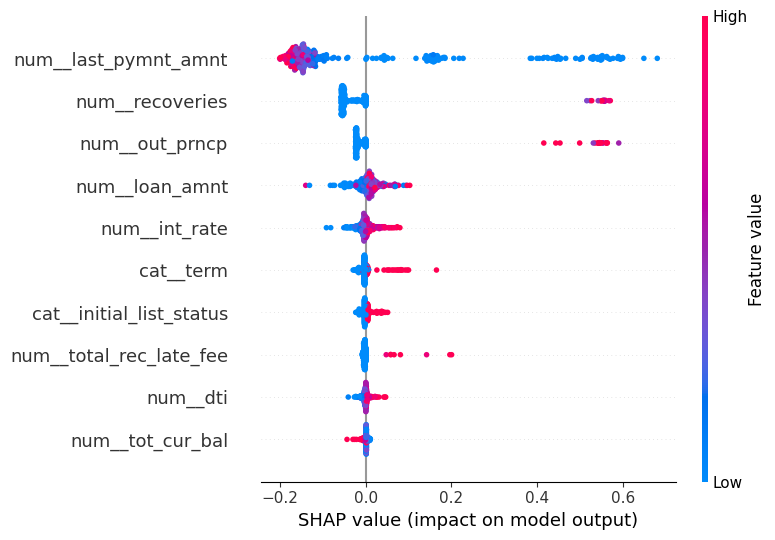
\includegraphics[width=0.85\textwidth]{./images/resumen_global_shap.png}
    \caption{SHAP Summary Plot de la Mejor Red Neuronal}
    \label{fig:shap_summary}
\end{figure}

\textit{Nota.} El summary plot de SHAP muestra la distribución del impacto de cada variable sobre las predicciones del modelo. Cada punto representa una observación individual, y su posición en el eje horizontal indica cuánto contribuyó esa variable a la predicción (valores positivos aumentan la probabilidad de incumplimiento, valores negativos la disminuyen). El color indica el valor de la variable: rojo para valores altos, azul para valores bajos.

El summary plot permite identificar patrones globales sobre cómo cada variable influye en las predicciones. El análisis detallado de esta visualización revela los siguientes hallazgos:

\textbf{1. \texttt{num\_\_last\_pymnt\_amnt} (último pago recibido):} Es claramente la variable más importante del modelo. Se observa que los valores bajos (azul) generan impactos positivos grandes sobre la predicción, mientras que los valores altos (rojo) generan impactos negativos. Esto significa que los clientes que realizan pagos finales altos tienen menor riesgo de incumplimiento, mientras que aquellos con pagos finales bajos presentan un riesgo significativamente mayor. La dispersión vertical de los puntos indica que el efecto de esta variable es consistente en toda la población.

\textbf{2. \texttt{num\_\_recoveries} (recuperaciones):} Esta variable muestra un impacto muy elevado. Los valores altos de recuperaciones producen contribuciones SHAP positivas muy grandes, desplazando fuertemente la predicción hacia la clase de incumplimiento. La existencia de recuperaciones de deuda es, por tanto, un indicador fuerte de que el préstamo ya ha experimentado problemas de pago, lo que naturalmente aumenta la probabilidad de clasificación como incumplido.

\textbf{3. \texttt{num\_\_out\_prncp} (capital pendiente):} Los valores altos de capital pendiente desplazan la predicción hacia la clase de incumplimiento. Un saldo pendiente elevado puede indicar que el prestatario está al inicio del plazo del préstamo o que tiene dificultades para reducir el saldo, ambas situaciones asociadas con mayor riesgo crediticio.

\textbf{4. \texttt{num\_\_loan\_amnt} (monto del préstamo):} Esta variable muestra una influencia moderada. Los préstamos de mayor monto afectan la predicción, pero en menor medida que las tres variables anteriores. El efecto es interpretable: préstamos más grandes pueden representar mayor exposición y, por tanto, mayor riesgo.

\textbf{5. \texttt{num\_\_int\_rate} (tasa de interés):} La tasa de interés tiene un efecto relevante. Tasas más altas se asocian con mayor probabilidad de incumplimiento, lo que es consistente con la práctica financiera de asignar tasas más altas a prestatarios percibidos como más riesgosos.

\textbf{6. \texttt{cat\_\_term} (plazo del préstamo):} Los plazos largos (60 meses) generan impactos positivos, lo que indica que los préstamos con plazos más extensos presentan mayor incertidumbre y riesgo de incumplimiento.

Las variables \texttt{total\_rec\_late\_fee}, \texttt{dti} y \texttt{tot\_cur\_bal} muestran contribuciones existentes pero considerablemente menores, lo que confirma que su poder discriminante es secundario frente a las variables principales.

\begin{figure}[htbp]
    \centering
    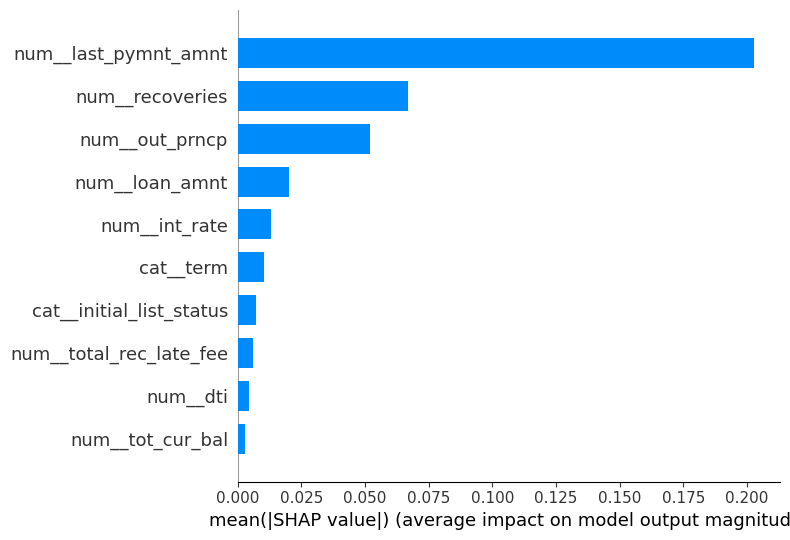
\includegraphics[width=0.85\textwidth]{./images/barplot_shap.png}
    \caption{SHAP Bar Plot de la Mejor Red Neuronal}
    \label{fig:shap_bar}
\end{figure}

\textit{Nota.} El bar plot de SHAP ordena las variables según su importancia global, calculada como el promedio de los valores absolutos de las contribuciones SHAP. Esta visualización proporciona un ranking claro de qué variables tienen mayor impacto en las predicciones del modelo.

El análisis SHAP del bar plot cuantifica la importancia global de cada variable. Los valores medios absolutos de SHAP revelan una jerarquía clara:

\begin{center}
\begin{tabular}{lc}
\toprule
Variable & Importancia SHAP (media \(|\)SHAP\(|\)) \\
\midrule
last\_pymnt\_amnt & 0.20 \\
recoveries        & 0.07 \\
out\_prncp        & 0.05 \\
loan\_amnt        & 0.02 \\
int\_rate         & 0.015 \\
\bottomrule
\end{tabular}
\end{center}

Estos valores confirman que existe una diferencia abismal entre la primera variable y el resto: \texttt{last\_pymnt\_amnt} tiene una importancia aproximadamente tres veces mayor que \texttt{recoveries} y cuatro veces mayor que \texttt{out\_prncp}. Esto indica que el modelo depende fuertemente del último pago recibido para generar sus predicciones.

El análisis SHAP confirma y refina los hallazgos del análisis exploratorio. Las variables más influyentes según SHAP son consistentes con las identificadas en el análisis de importancia de Random Forest (sección~\ref{sec:importancia}), lo que fortalece la validez de los hallazgos al obtener resultados convergentes desde dos metodologías independientes. Sin embargo, SHAP aporta información adicional al mostrar no solo qué variables son importantes, sino también la dirección y magnitud de su influencia en cada predicción individual.

Los resultados de SHAP revelan que \texttt{last\_pymnt\_amnt} (último pago recibido) es la variable con mayor impacto en las predicciones. Cuando el último pago es bajo, la contribución SHAP es positiva, lo que aumenta la probabilidad de incumplimiento. Cuando el último pago es alto, la contribución es negativa, lo que disminuye la probabilidad de incumplimiento. Este patrón es consistente con la intuición financiera: el comportamiento de pago reciente es un indicador fuerte del estado financiero del prestatario.

\texttt{recoveries} (recuperaciones post-incumplimiento) es la segunda variable más importante. Las recuperaciones altas indican que el préstamo ya ha entrado en proceso de cobranza o incumplimiento parcial, lo que naturalmente aumenta la probabilidad de que el modelo clasifique el caso como incumplido.

\texttt{out\_prncp} (capital pendiente) también figura entre las variables más influyentes. Un capital pendiente alto puede indicar que el prestatario está al inicio del plazo del préstamo o que tiene dificultades para reducir el saldo, ambas situaciones asociadas con mayor riesgo.

\texttt{int\_rate} (tasa de interés) muestra un patrón interesante: tasas de interés más altas están asociadas con mayor probabilidad de incumplimiento, lo que es consistente con la práctica financiera de asignar tasas más altas a prestatarios percibidos como más riesgosos.

El valor de SHAP radica en que no solo proporciona una explicación global del modelo, sino que también permite explicar predicciones individuales. Esto significa que, para cada solicitud de préstamo evaluada por el sistema, es posible generar un reporte detallado que explique qué factores influyeron más en la decisión y en qué dirección. Esta transparencia es fundamental para la adopción del sistema en un entorno financiero real, donde las decisiones deben ser justificables y auditables.

\subsection{Consideración sobre Posible Fuga de Información (\textit{Data Leakage})}

El análisis SHAP revela un hallazgo que merece una discusión crítica: la dominancia casi absoluta de variables como \texttt{last\_pymnt\_amnt}, \texttt{recoveries} y \texttt{out\_prncp} en las predicciones del modelo plantea la posibilidad de fuga de información (\textit{data leakage}). Estas variables suelen conocerse únicamente después de que el préstamo ya ha evolucionado en el tiempo ---es decir, después de que el prestatario ha realizado (o dejado de realizar) pagos, después de que se han generado recuperaciones, o después de que el capital pendiente ha sido calculado en un punto específico del ciclo de vida del préstamo.

Si el objetivo del modelo fuera predecir el riesgo crediticio en el momento de la solicitud (antes de otorgar el crédito), la inclusión de estas variables introduciría información futura que no estaría disponible en ese escenario, lo que invalidaría las predicciones para su uso en originación. Sin embargo, como se discutió en la sección~\ref{sec:limpieza}, el modelo fue diseñado explícitamente para tareas de monitoreo de cartera y cobranza temprana, donde estas variables sí están disponibles una vez que el préstamo ha sido desembolsado y ha transcurrido un período de observación.

Desde esta perspectiva, la dominancia de estas variables en el análisis SHAP no constituye un defecto del modelo, sino una confirmación de que el sistema captura efectivamente las señales de deterioro crediticio que se manifiestan durante la vida del préstamo. No obstante, es fundamental que los usuarios del sistema comprendan esta limitación: el modelo es adecuado para evaluar el riesgo de préstamos ya originados, pero no para evaluar solicitudes nuevas donde estas variables no están disponibles.

% ═══════════════════════════════════════════════
% 6. RESULTADOS Y EVALUACIÓN COMPARATIVA
% ═══════════════════════════════════════════════
\section{Resultados y Evaluación Comparativa}
\label{sec:resultados}

La evaluación del desempeño del modelo es una etapa crítica del proyecto, ya que permite determinar si el sistema cumple con los objetivos planteados y si es adecuado para su uso en un entorno real. En este proyecto, la evaluación se realizó comparando el desempeño de la red neuronal contra una línea base de regresión logística, utilizando múltiples métricas que capturan diferentes aspectos del rendimiento del modelo.

\subsection{Métricas de Evaluación}

Para comprender los resultados, es necesario primero entender qué mide cada métrica y por qué es relevante en el contexto de riesgo crediticio.

\textbf{PR-AUC (Área Bajo la Curva Precision-Recall):} Esta métrica evalúa la capacidad del modelo para identificar correctamente los casos positivos (incumplimiento) manteniendo una alta precisión. Es particularmente útil cuando se trabaja con clases desbalanceadas, como es el caso de este proyecto, donde la clase de incumplimiento representa aproximadamente el 23\% de los datos. Un PR-AUC alto indica que el modelo es capaz de detectar la mayoría de los casos de incumplimiento sin generar demasiados falsos positivos.

\textbf{ROC-AUC (Área Bajo la Curva ROC):} Esta métrica evalúa la capacidad del modelo para distinguir entre las dos clases en todos los umbrales de decisión posibles. Un ROC-AUC de 1.0 indica un modelo perfecto, mientras que un valor de 0.5 indica un modelo que no distingue entre las clases. El ROC-AUC es una medida general del desempeño del modelo, independiente del umbral de decisión específico.

\textbf{Precisión:} De todos los casos que el modelo clasificó como incumplimiento, ¿cuántos realmente eran incumplimientos? Una precisión alta significa que cuando el modelo predice incumplimiento, es muy probable que efectivamente lo sea.

\textbf{Recall (Sensibilidad):} De todos los casos reales de incumplimiento, ¿cuántos logró detectar el modelo? Un recall alto significa que el modelo es capaz de identificar la mayoría de los casos de incumplimiento, lo cual es crucial en el contexto financiero, donde no detectar un caso de incumplimiento puede tener consecuencias graves.

\textbf{F1-Score:} Es el promedio armónico de la precisión y el recall, proporcionando una medida balanceada del desempeño del modelo en la clase de interés.

\textbf{Accuracy (Exactitud):} De todos los casos evaluados, ¿cuántos fueron clasificados correctamente? Aunque es una métrica útil, puede ser engañosa cuando se trabaja con clases desbalanceadas, ya que un modelo que siempre prediga la clase mayoritaria podría tener un accuracy alto sin ser útil para detectar la clase minoritaria.

\subsection{Resultados Comparativos}

La siguiente tabla presenta los resultados obtenidos por la red neuronal y la regresión logística en el conjunto de prueba:

\begin{table}[htbp]
    \centering
    \caption{Comparación de Desempeño entre Modelos}
    \label{tab:resultados}
    \small
    \begin{tabular}{lccccc}
        \toprule
        Modelo & PR-AUC (Prueba) & Accuracy & F1 Clase 1 & Precisión Clase 1 & Recall Clase 1 \\
        \midrule
        Red Neuronal        & 0.9831 & 0.9532 & 0.9062 & 0.8409 & 0.9824 \\
        Regresión Logística & 0.9603 & 0.9326 & 0.8681 & 0.7907 & 0.9624 \\
        \bottomrule
    \end{tabular}
\end{table}

\textit{Nota.} La tabla muestra las métricas principales de desempeño para ambos modelos en el conjunto de prueba. Los valores más altos en cada métrica indican mejor desempeño.

Los resultados muestran claramente que la red neuronal supera a la regresión logística en todas las métricas evaluadas. Esta diferencia es particularmente notable en el PR-AUC, donde la red neuronal alcanza un valor de 0.9831 frente a 0.9603 de la regresión logística. Esta mejora de más de 2 puntos porcentuales es significativa, especialmente considerando que el PR-AUC es la métrica más relevante para problemas con clases desbalanceadas.

En términos de accuracy global, la red neuronal logra un 95.32\% de clasificaciones correctas, frente al 93.26\% de la regresión logística. Aunque esta diferencia puede parecer pequeña, representa una mejora sustancial en el contexto de más de 38,000 evaluaciones realizadas en el conjunto de prueba.

Donde la diferencia es más crítica es en el recall de la clase de incumplimiento. La red neuronal logra detectar el 98.24\% de los casos reales de incumplimiento, mientras que la regresión logística detecta el 96.24\%. Esta diferencia de 2 puntos porcentuales significa que la red neuronal es capaz de identificar aproximadamente 175 casos adicionales de incumplimiento que la regresión logística habría pasado por alto. En el contexto financiero, donde cada caso de incumplimiento no detectado representa una pérdida potencial, esta mejora es significativa.

La precisión de la clase de incumplimiento también es superior en la red neuronal (84.09\% vs 79.07\%), lo que significa que cuando el modelo predice incumplimiento, es más probable que efectivamente lo sea. Esto reduce el número de falsos positivos, es decir, casos que el modelo clasifica erróneamente como incumplimientos cuando en realidad son préstamos cumplidos.

\subsection{Análisis Visual del Desempeño del Modelo}

Complementando las métricas cuantitativas presentadas anteriormente, se generaron cuatro visualizaciones clave que permiten evaluar el comportamiento del modelo desde perspectivas adicionales: la dinámica del entrenamiento, la distribución de aciertos y errores, la capacidad discriminante global, y el rendimiento bajo condiciones de desbalance de clases.

\subsubsection{Dinámica de Entrenamiento: Curvas de Pérdida}

\begin{figure}[htbp]
    \centering
    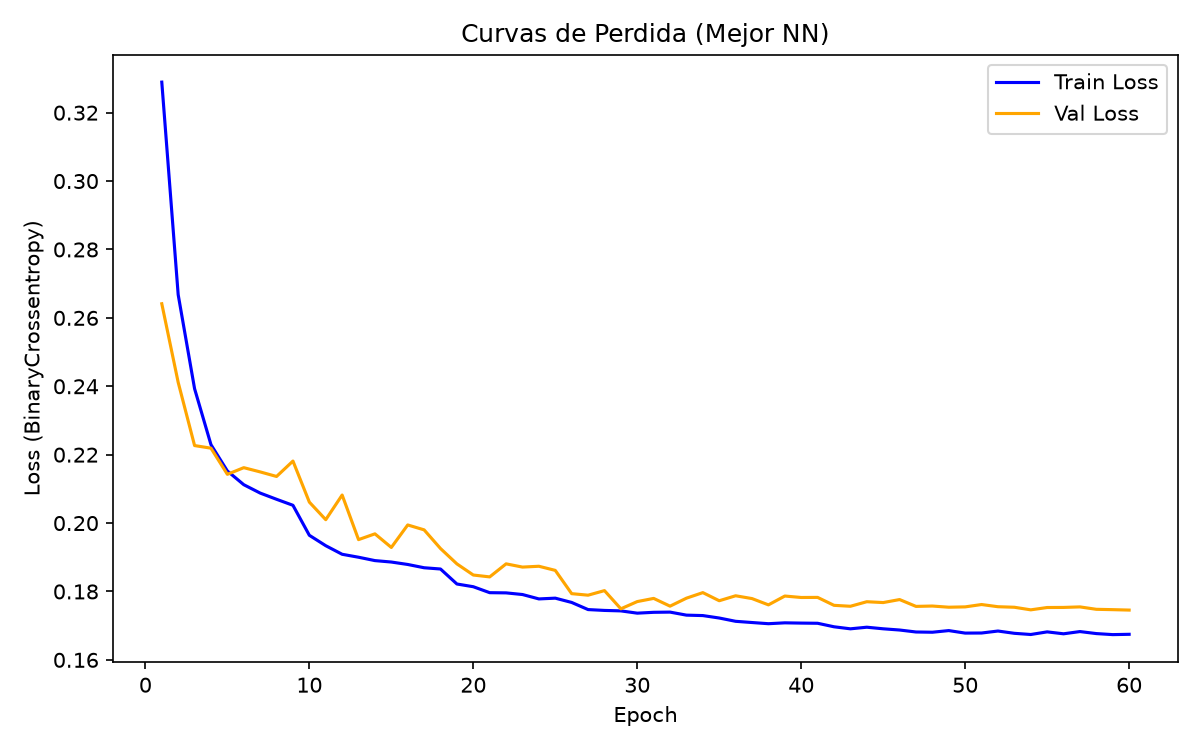
\includegraphics[width=0.85\textwidth]{./images/loss_curves.png}
    \caption{Curvas de Pérdida (Binary Crossentropy) durante el Entrenamiento}
    \label{fig:loss}
\end{figure}

\textit{Nota.} Evolución de la función de pérdida Binary Crossentropy a lo largo de 60 épocas de entrenamiento, tanto para el conjunto de entrenamiento (Train Loss) como para el conjunto de validación (Val Loss). La cercanía entre ambas curvas a lo largo de todo el entrenamiento indica que el modelo generaliza correctamente sin presentar sobreajuste.

La Figura~\ref{fig:loss} muestra la evolución de la función de pérdida (Binary Crossentropy) a lo largo de 60 épocas de entrenamiento, tanto para el conjunto de entrenamiento como para el de validación. El análisis de estas curvas proporciona información fundamental sobre la dinámica de aprendizaje del modelo:

\textbf{Comportamiento de las curvas:} Ambas curvas decrecen de forma pronunciada durante las primeras 10 épocas, lo que indica un aprendizaje rápido y eficiente en la fase inicial del entrenamiento. Esta caída acelerada refleja que el modelo logra capturar rápidamente los patrones más evidentes que distinguen a los prestatarios cumplidos de los incumplidos.

\textbf{Estabilización y convergencia:} Alrededor de la época 30, las curvas comienzan a aplanarse progresivamente. Hacia el final del entrenamiento (época 60), el Train Loss se estabiliza cerca de 0.167 y el Val Loss cerca de 0.174, lo que indica que el modelo ha convergido hacia un mínimo estable de la función de pérdida.

\textbf{Diagnóstico de sobreajuste:} La brecha (\textit{gap}) entre la pérdida de entrenamiento y la de validación es extremadamente pequeña y se mantiene paralela a lo largo de todo el entrenamiento. Esta es una excelente señal: el modelo tiene una gran capacidad de generalización y no presenta problemas significativos de sobreajuste (\textit{overfitting}). La regularización L1, el dropout de 0.5 y la normalización por lotes ---combinados con los mecanismos de detención temprana y reducción de la tasa de aprendizaje--- resultaron efectivos para controlar la complejidad del modelo durante el entrenamiento.

\subsubsection{Distribución de Aciertos y Errores: Matriz de Confusión}

\begin{figure}[htbp]
    \centering
    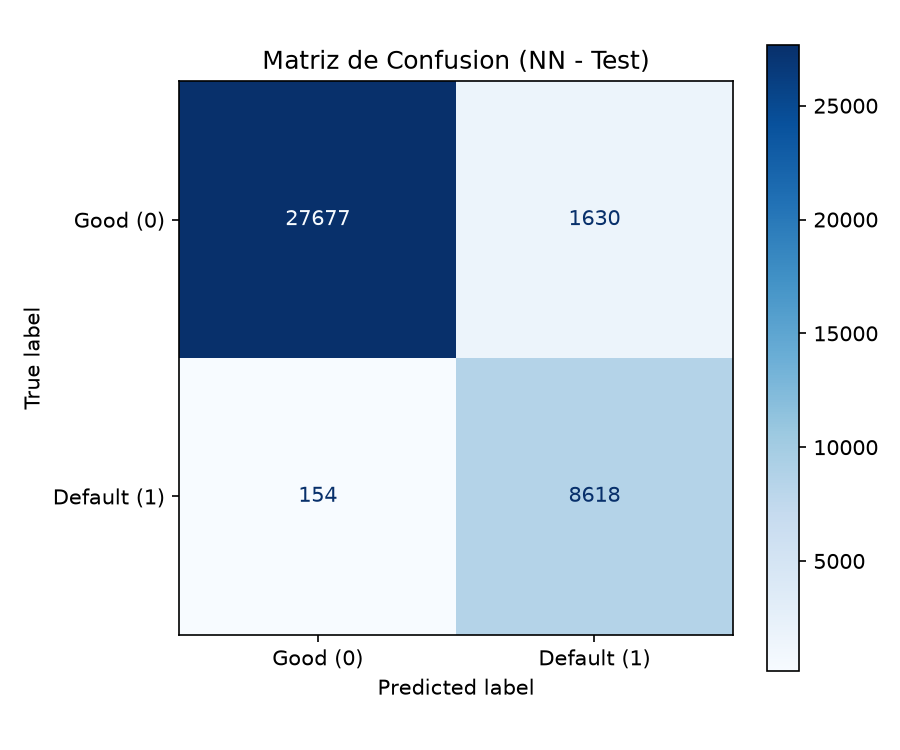
\includegraphics[width=0.75\textwidth]{./images/confusion_matrix.png}
    \caption{Matriz de Confusión en el Conjunto de Prueba}
    \label{fig:confusion}
\end{figure}

\textit{Nota.} Matriz de confusión que muestra la distribución de las predicciones del modelo en el conjunto de prueba, clasificando los clientes entre Good (0) ---buenos pagadores--- y Default (1) ---clientes en impago---. Los valores de la diagonal principal representan clasificaciones correctas, mientras que los valores fuera de la diagonal representan errores de clasificación.

La matriz de confusión (Figura~\ref{fig:confusion}) evalúa el desempeño del modelo en el conjunto de prueba, proporcionando un desglose detallado de los aciertos y errores por clase. A partir del reporte de clasificación del modelo se derivan las siguientes métricas:

\textbf{Exactitud (Accuracy):} La proporción de clasificaciones correctas sobre el total de evaluaciones es de 95.32\%. Este valor confirma el alto nivel de acierto global del modelo.

\textbf{Sensibilidad / Exhaustividad (Recall para Default):} El modelo es capaz de detectar al 98.24\% de las personas que van a caer en impago. Desde la perspectiva del negocio, esto es crucial para el análisis de riesgo: el sistema identifica prácticamente a la totalidad de los clientes que presentarán problemas de pago, permitiendo a la institución financiera tomar acciones preventivas de manera oportuna.

\textbf{Precisión (Precision para Default):} Cuando el modelo genera una alerta de Default, tiene un 84.09\% de acierto. Esto significa que un 15.91\% de las alertas generadas son falsas alarmas ---clientes buenos que son bloqueados o enviados a revisión manual---. Si bien este porcentaje representa un costo operativo asociado a la gestión de falsos positivos, es un trade-off aceptable en el contexto de riesgo crediticio, donde el costo de no detectar un caso de incumplimiento suele ser significativamente mayor que el costo de revisar manualmente un falso positivo.

\subsubsection{Capacidad Discriminante Global: Curva ROC}

\begin{figure}[htbp]
    \centering
    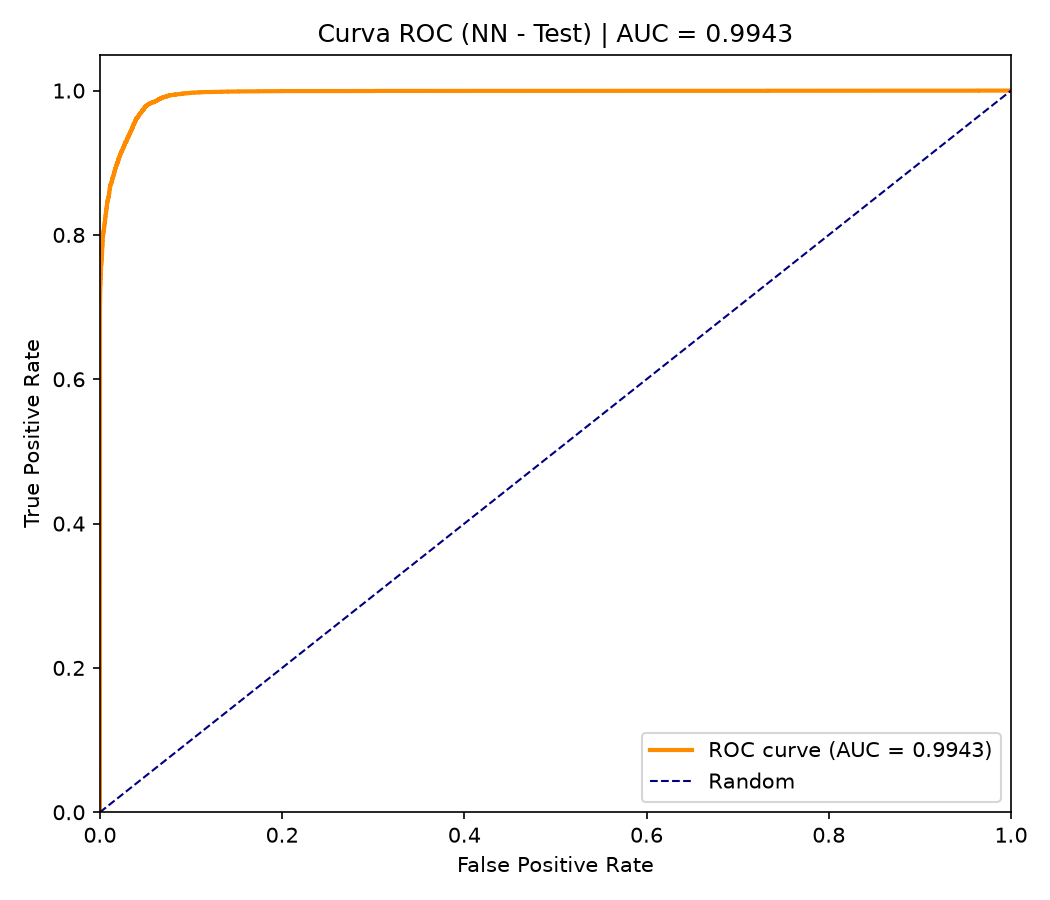
\includegraphics[width=0.75\textwidth]{./images/roc_auc_curve.png}
    \caption{Curva ROC (Receiver Operating Characteristic)}
    \label{fig:roc}
\end{figure}

\textit{Nota.} Curva ROC que contrasta la tasa de verdaderos positivos (True Positive Rate) frente a la tasa de falsos positivos (False Positive Rate) a distintos umbrales de decisión. El área bajo la curva (AUC) cuantifica la capacidad global del modelo para discriminar entre las dos clases. La línea diagonal punteada representa el desempeño de un clasificador aleatorio.

La curva ROC (Figura~\ref{fig:roc}) proporciona una evaluación comprehensiva de la capacidad del modelo para discriminar entre las dos clases a lo largo de todos los umbrales de decisión posibles.

\textbf{Métrica AUC:} El área bajo la curva es de 0.9943, un valor excepcionalmente cercano al máximo teórico de 1.0.

\textbf{Interpretación:} Un AUC de 0.9943 representa un rendimiento casi perfecto en cuanto a la capacidad del modelo para separar o discriminar entre las dos clases ---saber quién es solvente y quién no---. La curva se eleva de manera casi vertical hacia la esquina superior izquierda, alejándose drásticamente de la línea diagonal de clasificación aleatoria (AUC = 0.5). Esto significa que, para prácticamente cualquier umbral de decisión, el modelo logra mantener una tasa de verdaderos positivos muy alta con una tasa de falsos positivos muy baja.

Este resultado complementa y contextualiza el PR-AUC reportado en la Tabla~\ref{tab:resultados}. Mientras que el ROC-AUC de 0.9943 evalúa el desempeño global del modelo en todos los umbrales, el PR-AUC se enfoca específicamente en el rendimiento sobre la clase minoritaria (incumplimiento). La convergencia de ambas métricas hacia valores cercanos a 1.0 confirma la solidez del modelo.

\subsubsection{Rendimiento bajo Desbalance de Clases: Curva Precision-Recall}

\begin{figure}[htbp]
    \centering
    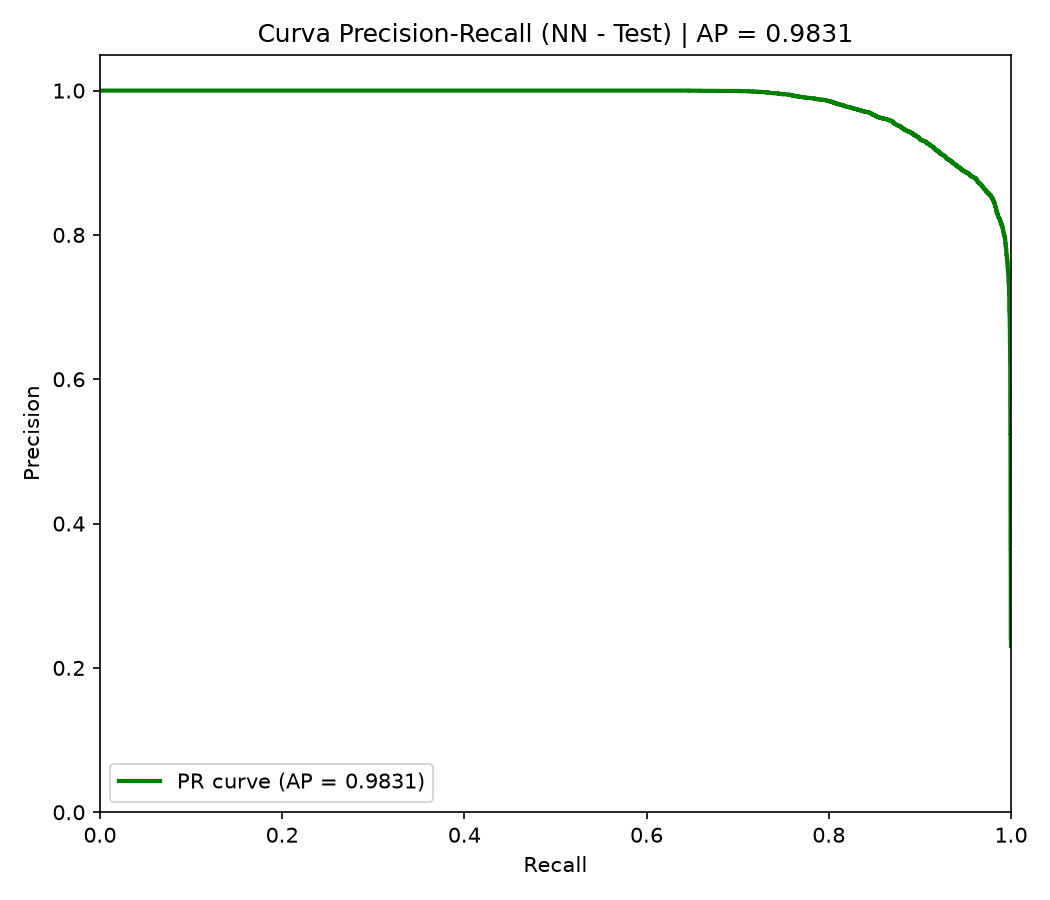
\includegraphics[width=0.75\textwidth]{./images/precision_recall_curve.png}
    \caption{Curva Precision-Recall}
    \label{fig:pr}
\end{figure}

\textit{Nota.} Curva Precision-Recall que muestra la relación entre la precisión (Precision) y la exhaustividad (Recall) a distintos umbrales de decisión. Dado que en problemas de riesgo crediticio las clases suelen estar desbalanceadas, esta curva constituye la métrica más rigurosa para evaluar el desempeño del modelo sobre la clase de interés (Default). El valor de Average Precision (AP) resume el rendimiento global de la curva.

En problemas de riesgo crediticio y detección de fraudes, las clases suelen estar desbalanceadas ---en este dataset, la clase de incumplimiento representa aproximadamente el 23\% de los registros---. En este contexto, la curva Precision-Recall es considerada la métrica más honesta y rigurosa, ya que se enfoca exclusivamente en el desempeño del modelo sobre la clase minoritaria, sin verse influida por el alto número de verdaderos negativos de la clase mayoritaria.

\textbf{Métrica AP (Average Precision):} El modelo alcanza un valor de 0.9831, es decir, un 98.31\% de precisión promedio.

\textbf{Interpretación:} Un AP de 98.31\% confirma que el rendimiento es sobresaliente incluso bajo la lupa más exigente de la precisión y el recall combinados. La curva se mantiene plana en la parte superior (Precision = 1.0) durante casi todo el recorrido del Recall, y solo empieza a decaer levemente cuando el Recall supera el 80\%--90\%. Esto demuestra que el modelo mantiene una alta fidelidad ---generando muy pocos falsos positivos--- a pesar de capturar a casi la totalidad de los clientes en default.

Este resultado es particularmente relevante porque valida que el alto recall del modelo (98.24\%) no se logra a costa de una precisión deteriorada. El modelo logra un equilibrio excepcional entre detectar la mayor cantidad posible de casos de incumplimiento y mantener la calidad de las alertas generadas, lo cual es esencial para la viabilidad operativa del sistema en un entorno financiero real.

\subsection{Interpretación de los Resultados desde la Perspectiva de Negocio}

Los resultados obtenidos demuestran que la red neuronal no solo es técnicamente superior a la regresión logística, sino que también es más adecuada para los objetivos del proyecto. En el contexto de monitoreo de cartera y cobranza temprana, el objetivo principal es identificar la mayor cantidad posible de casos de incumplimiento, incluso si esto implica aceptar un número moderado de falsos positivos.

El alto recall de la red neuronal (98.24\%) significa que el sistema es capaz de detectar casi todos los casos de incumplimiento, lo que permite a la institución financiera tomar acciones preventivas de manera oportuna. Esto puede incluir contacto temprano con el prestatario, oferta de reestructuración de deuda, o asignación prioritaria a equipos de cobranza.

Al mismo tiempo, la precisión de 84.09\% indica que la mayoría de las alertas generadas por el sistema son legítimas, lo que reduce el costo operativo asociado con la gestión de falsos positivos. En términos prácticos, esto significa que los equipos de cobranza pueden enfocarse en los casos que realmente lo necesitan, mejorando la eficiencia operativa.

El PR-AUC de 0.9831 es excepcionalmente alto y demuestra que el modelo tiene una capacidad sobresaliente para distinguir entre préstamos cumplidos e incumplidos. Este nivel de desempeño es consistente con los mejores resultados reportados en la literatura académica sobre credit scoring (Lessmann et al., 2015).

Es importante destacar que el umbral de decisión fue optimizado para maximizar el F2-score, una métrica que pondera más el recall que la precisión. Esto refleja una política de detección sensible, orientada a priorizar la identificación de casos riesgosos sobre la minimización de falsos positivos. El umbral óptimo de 0.54933 (ligeramente superior al valor por defecto de 0.5) ajusta la sensibilidad del modelo para equilibrar la detección de incumplimientos con la precisión de las predicciones.

\subsection{Limitaciones de la Evaluación}

Aunque los resultados son sólidos, es importante reconocer algunas limitaciones de la evaluación realizada. En primer lugar, el conjunto de datos utilizado proviene de una plataforma específica de préstamos peer-to-peer (LendingClub), lo que puede limitar la generalización de los resultados a otros contextos financieros o a diferentes tipos de préstamos.

En segundo lugar, como se discutió anteriormente, el conjunto de variables utilizadas incluye información posterior al desembolso del préstamo. Esto significa que el modelo es más adecuado para tareas de monitoreo de cartera que para la evaluación de solicitudes iniciales. Esta es una limitación metodológica importante que debe considerarse al interpretar los resultados y al planificar la implementación del sistema en un entorno real.

En tercer lugar, aunque el modelo fue evaluado en un conjunto de prueba independiente, no se realizó una validación temporal que simule el desempeño del modelo en el tiempo. En la práctica, los patrones de riesgo crediticio pueden cambiar debido a factores macroeconómicos, cambios en las políticas de crédito, o evoluciones en el comportamiento de los prestatarios. Una evaluación robusta debería incluir pruebas de estabilidad temporal para asegurar que el modelo mantiene su desempeño a lo largo del tiempo.

% ═══════════════════════════════════════════════
% 7. SCORECARD Y APLICACIÓN WEB
% ═══════════════════════════════════════════════
\section{Scorecard y Aplicación Web}

\subsection{Del Modelo a la Aplicación Práctica: El Scorecard}

El desarrollo de un modelo predictivo es solo el primer paso hacia la creación de una solución completa. Para que el modelo genere valor real, debe ser integrado en una aplicación práctica que permita a los usuarios finales utilizar sus predicciones de manera intuitiva y efectiva. En este proyecto, se desarrolló una aplicación web que transforma las predicciones del modelo en un score crediticio fácil de interpretar.

El scorecard implementado convierte la probabilidad de incumplimiento generada por el modelo en una puntuación numérica en una escala de 300 a 850, similar a las escalas utilizadas por las agencias de crédito tradicionales como FICO. Es importante aclarar que esta transformación corresponde a un mapeo lineal simplificado y no a un scorecard estadístico convencional basado en \textit{odds mapping} y asignación ponderada de puntos por variable. La conversión sigue una regla de transformación lineal simple:

\[
\text{Score} = 850 - (\text{Probabilidad de Incumplimiento} \times 550)
\]

Bajo esta lógica, una probabilidad de incumplimiento de 0 (cero riesgo) se traduce en un score de 850, mientras que una probabilidad de 1 (certeza de incumplimiento) se traduce en un score de 300. Esta escala inversamente proporcional al riesgo es intuitiva para los usuarios: un score más alto indica menor riesgo, mientras que un score más bajo indica mayor riesgo.

El scorecard no solo facilita la interpretación de las predicciones, sino que también permite establecer umbrales de decisión claros. Por ejemplo, una institución financiera podría definir que solicitudes con score superior a 650 se aprueban automáticamente, solicitudes con score entre 500 y 650 requieren revisión manual, y solicitudes con score inferior a 500 se rechazan. Esta estandarización agiliza el proceso de toma de decisiones y reduce la subjetividad.

\subsection{La Aplicación Web: Interfaz para el Usuario Final}

Para hacer el modelo accesible a los usuarios finales, se desarrolló una aplicación web que permite ingresar las características de un préstamo y obtener una predicción de riesgo en tiempo real. La aplicación está construida con tecnologías modernas de desarrollo web y se comunica con el modelo a través de una API RESTful desarrollada con FastAPI.

\begin{figure}[htbp]
    \centering
    
\includegraphics[width=0.9\textwidth]{./images/webapp.png}
    \caption{Interfaz de la Aplicación Web de Predicción de Riesgo Crediticio}
    \label{fig:webapp}
\end{figure}

\textit{Nota.} Captura de pantalla de la aplicación web que muestra el formulario de entrada de datos y la visualización de resultados, incluyendo el score crediticio, la probabilidad de incumplimiento, y la importancia de las variables en la predicción.

La aplicación web incluye varios componentes diseñados para mejorar la experiencia del usuario y facilitar la interpretación de los resultados:

\textbf{Formulario de entrada:} Permite al usuario ingresar las características del préstamo o del prestatario. Los campos incluyen el monto del préstamo, la tasa de interés, el plazo, el último pago recibido, las recuperaciones, el capital pendiente, los cargos por mora, el saldo total actual, la relación deuda-ingresos, y el estatus inicial en lista. La interfaz está diseñada para ser intuitiva y guiar al usuario en el ingreso de los datos.

\textbf{Visualización del score:} Un medidor visual (gauge) muestra el score crediticio en la escala de 300 a 850, con indicadores de color que facilitan la interpretación: verde para scores altos (bajo riesgo), amarillo para scores medios (riesgo moderado), y rojo para scores bajos (alto riesgo). Esta visualización permite al usuario comprender rápidamente el nivel de riesgo asociado a la solicitud.

\textbf{Probabilidad de incumplimiento:} Además del score, la aplicación muestra la probabilidad de incumplimiento estimada por el modelo, expresada como un porcentaje. Esta información complementa el score y proporciona una medida más directa del riesgo.

\textbf{Importancia de variables:} La aplicación incluye una visualización que muestra qué variables influyeron más en la predicción y en qué dirección. Esta información es crucial para la transparencia del sistema, ya que permite al usuario comprender los factores que llevaron a esa clasificación de riesgo específica.

\textbf{Gráfico de población:} Una visualización adicional muestra dónde se ubica la solicitud evaluada en relación con la distribución de riesgo de la población total. Esto permite contextualizar el resultado y comprender si el riesgo es alto o bajo en términos relativos.

\subsection{Valor para el Usuario Final}

La aplicación web transforma un modelo técnico complejo en una herramienta práctica y accesible para la toma de decisiones financieras. Su valor radica en varios aspectos:

\textbf{Rapidez:} La evaluación de una solicitud que tradicionalmente podría tomar horas o días se realiza en segundos, permitiendo una respuesta inmediata al cliente.

\textbf{Consistencia:} A diferencia de la evaluación manual, que puede variar según el analista, el modelo proporciona evaluaciones consistentes basadas en los mismos criterios objetivos.

\textbf{Transparencia:} La aplicación no solo proporciona una predicción, sino que también explica los factores que influyeron en esa predicción, lo que facilita la justificación de las decisiones ante los clientes y los reguladores.

\textbf{Escalabilidad:} El sistema puede procesar múltiples solicitudes simultáneamente, lo que permite a las instituciones financieras manejar grandes volúmenes de evaluaciones sin incrementar proporcionalmente sus recursos.

\textbf{Accesibilidad:} Al estar disponible como aplicación web, el sistema puede ser accedido desde cualquier lugar y en cualquier momento, facilitando su integración en los procesos de negocio existentes.

Para las instituciones financieras, esta herramienta representa una mejora significativa en la capacidad de evaluar y monitorear el riesgo crediticio. Para los analistas de riesgo, proporciona una herramienta de apoyo a la decisión que complementa su juicio experto. Para los clientes, significa evaluaciones más rápidas, justas y transparentes.

% ═══════════════════════════════════════════════
% 8. CONCLUSIONES, APRENDIZAJES Y LIMITACIONES
% ═══════════════════════════════════════════════
\section{Conclusiones, Aprendizajes y Limitaciones}

\subsection{Conclusiones Principales}

El proyecto demostró que es posible desarrollar un sistema de predicción de riesgo crediticio basado en redes neuronales profundas que supere significativamente a los métodos tradicionales como la regresión logística. Los resultados obtenidos muestran que la red neuronal no solo es más precisa en términos generales, sino que también es superior en la detección de casos de incumplimiento, que es el objetivo principal del sistema.

La combinación de un PR-AUC de 0.9831, un ROC-AUC de 0.9943, un Average Precision de 0.9831, y un recall de 0.9824 para la clase de incumplimiento demuestra que el modelo es capaz de identificar casi todos los casos de incumplimiento manteniendo una alta precisión. Las curvas de pérdida confirman además que el entrenamiento convergió de manera estable sin presentar sobreajuste, con una brecha mínima entre la pérdida de entrenamiento y validación. Este nivel de desempeño es excepcional y está en línea con los mejores resultados reportados en la literatura académica sobre credit scoring.

Más allá del aspecto técnico, el proyecto demostró que es posible crear una solución completa que va desde el análisis de datos hasta la implementación de una aplicación web práctica. La integración del modelo en una interfaz amigable, con visualizaciones claras y explicaciones transparentes, convierte un modelo técnico complejo en una herramienta útil para la toma de decisiones financieras.

El análisis de interpretabilidad mediante SHAP permitió comprender cómo el modelo utiliza las variables para generar sus predicciones, abordando uno de los principales desafíos de las redes neuronales: la falta de transparencia. Esta capacidad de explicación es fundamental para la adopción del sistema en un entorno financiero real, donde las decisiones deben ser justificables y auditables.

\subsection{Aprendizajes Clave}

El desarrollo del proyecto dejó varios aprendizajes importantes que vale la pena destacar:

\textbf{La calidad de los datos es fundamental:} La etapa de limpieza y preparación de datos fue determinante para el éxito del modelo. La eliminación de variables con valores faltantes elevados, la identificación de variables redundantes, y la selección cuidadosa del conjunto final de variables permitieron reducir el ruido y mejorar la calidad de las predicciones. Sin este trabajo previo, el modelo habría tenido un desempeño significativamente inferior.

\textbf{El manejo del desbalance de clases requiere estrategias específicas:} En problemas donde una clase es mucho menos frecuente que la otra, como es el caso del incumplimiento crediticio, es necesario utilizar estrategias como la ponderación de clases y el ajuste del umbral de decisión para evitar que el modelo favorezca en exceso a la clase mayoritaria. La optimización del umbral mediante el F2-score permitió desplazar la decisión hacia una mayor sensibilidad sobre la clase de incumplimiento, que es el objetivo principal del sistema.

\textbf{La interpretabilidad es tan importante como la precisión:} Un modelo preciso pero incomprensible tiene limitada utilidad en el contexto financiero. La implementación de SHAP permitió no solo explicar las predicciones del modelo, sino también validar que los factores identificados como importantes son consistentes con el conocimiento del dominio y con los hallazgos del análisis exploratorio.

\textbf{La delimitación del problema es crucial:} Una de las decisiones más importantes del proyecto fue reconocer que el conjunto de variables utilizadas incluye información posterior al desembolso del préstamo, lo que significa que el modelo es más adecuado para tareas de monitoreo de cartera que para la evaluación de solicitudes iniciales. Esta delimitación evita sobrestimar el alcance del modelo y permite interpretarlo correctamente en su contexto adecuado.

\textbf{La comparación con líneas base es esencial:} La inclusión de una regresión logística como línea base permitió contextualizar los resultados y demostrar que la complejidad adicional de la red neuronal se traduce en una mejora tangible del desempeño. Sin esta comparación, no habría sido posible determinar si el uso de una red neuronal era realmente necesario o si un modelo más simple habría sido suficiente.

\subsection{Limitaciones y Trabajo Futuro}

Aunque el proyecto logró sus objetivos principales, es importante reconocer sus limitaciones y identificar áreas de mejora para trabajo futuro:

\textbf{Alcance del modelo:} Como se discutió anteriormente, el feature set final no corresponde a un escenario de originación pura, sino a un escenario de monitoreo de cartera post-desembolso. Esto limita la aplicabilidad del modelo para la evaluación de solicitudes iniciales. Un trabajo futuro podría enfocarse en desarrollar un modelo separado para originación, utilizando únicamente variables disponibles en el momento de la solicitud.

\textbf{Validación temporal:} El modelo fue evaluado en un conjunto de prueba estático, pero no se realizó una validación temporal que simule su desempeño a lo largo del tiempo. En la práctica, los patrones de riesgo crediticio pueden cambiar debido a factores macroeconómicos o cambios en el comportamiento de los prestatarios. Una evaluación robusta debería incluir pruebas de estabilidad temporal y mecanismos de actualización continua del modelo.

\textbf{Equidad y sesgo (Fairness):} No se realizó un análisis exhaustivo de equidad para evaluar si el modelo presenta sesgos diferenciales contra subgrupos demográficos protegidos (por ejemplo, por género, etnia o ubicación geográfica). En el contexto financiero, esta evaluación es fundamental para cumplir con regulaciones antidiscriminación y garantizar que las decisiones crediticias sean justas. Un trabajo futuro debería incorporar métricas de equidad (como \textit{equalized odds} o \textit{demographic parity}) y técnicas de mitigación de sesgo si se detectan disparidades.

\textbf{Generalización a otros contextos:} El modelo fue entrenado y evaluado en un dataset específico de préstamos peer-to-peer de LendingClub. Aunque los resultados son prometedores, no está claro cómo se desempeñaría el modelo en otros contextos financieros o con diferentes tipos de préstamos. Un trabajo futuro debería explorar la transferibilidad del modelo a otros datasets y contextos.

\textbf{Expansión del scorecard:} La implementación actual del scorecard es básica y utiliza una transformación lineal simple. Un trabajo futuro podría desarrollar un scorecard más sofisticado que incorpore factores de ajuste adicionales y que permita calibrar la escala de acuerdo con los estándares de la industria.

\textbf{Integración con sistemas existentes:} Aunque la aplicación web demuestra la viabilidad del enfoque, su integración con los sistemas de gestión de crédito existentes en las instituciones financieras requeriría trabajo adicional de ingeniería de software y cumplimiento normativo.

\subsection{Reflexión Final}

El proyecto representa un ejemplo completo de cómo la inteligencia artificial puede aplicarse para resolver problemas reales del sector financiero. Desde el análisis exploratorio de datos hasta la implementación de una aplicación web práctica, el proyecto demuestra que es posible construir sistemas de predicción de riesgo crediticio que no solo son técnicamente sólidos, sino también útiles, transparentes y accesibles para los usuarios finales.

Más allá de los resultados técnicos, el proyecto deja una lección importante: el éxito de un proyecto de ciencia de datos no depende únicamente de la calidad del modelo, sino también de la capacidad de comprender el problema de negocio, preparar cuidadosamente los datos, interpretar los resultados de manera crítica, y comunicar los hallazgos de manera efectiva a los stakeholders. La inteligencia artificial no es una solución mágica, sino una herramienta poderosa que, cuando se utiliza de manera responsable y contextualizada, puede aportar valor significativo a las organizaciones y a la sociedad en general.

% ═══════════════════════════════════════════════
% 9. REFERENCIAS BIBLIOGRÁFICAS
% ═══════════════════════════════════════════════
\section{Referencias Bibliográficas}

\begin{thebibliography}{99}

\bibitem{bcbs2020}
Basel Committee on Banking Supervision. (2020). \textit{Studies on the validation of internal ratings-based models} (revised). Bank for International Settlements. \url{https://www.bis.org/bcbs/publ/d494.pdf}

\bibitem{d0ubt0repo}
d0ubt0. (s.f.). \textit{credit-risk} [Repositorio de GitHub]. GitHub. Recuperado el 21 de abril de 2026, de \url{https://github.com/d0ubt0/credit-risk}

\bibitem{d0ubt0app}
d0ubt0. (s.f.). \textit{credit-risk-neuronal-network} [Aplicación web]. Netlify. Recuperado el 21 de abril de 2026, de \url{https://credit-risk-neuronal-network.netlify.app/}

\bibitem{goodfellow2016}
Goodfellow, I., Bengio, Y., \& Courville, A. (2016). \textit{Deep learning}. MIT Press. \url{https://www.deeplearningbook.org/}

\bibitem{kaggle}
Kaggle. (s.f.). \textit{Lending Club Loan Data}. Recuperado el 21 de abril de 2026, de \url{https://www.kaggle.com/datasets/laotse/credit-risk-dataset}

\bibitem{lecun2015}
LeCun, Y., Bengio, Y., \& Hinton, G. (2015). Deep learning. \textit{Nature, 521}(7553), 436--444. \url{https://doi.org/10.1038/nature14539}

\bibitem{lessmann2015}
Lessmann, S., Baesens, B., Seow, H.-V., \& Thomas, L. C. (2015). Benchmarking state-of-the-art classification algorithms for credit scoring: An update of research. \textit{European Journal of Operational Research, 247}(1), 124--136. \url{https://doi.org/10.1016/j.ejor.2015.05.030}

\bibitem{lundberg2017}
Lundberg, S. M., \& Lee, S.-I. (2017). A unified approach to interpreting model predictions. En I. Guyon et al. (Eds.), \textit{Advances in Neural Information Processing Systems 30 (NeurIPS 2017)}. \url{https://proceedings.neurips.cc/paper_files/paper/2017/file/8a20a8621978632d76c43dfd28b67767-Paper.pdf}

\bibitem{mishkin2019}
Mishkin, F. S. (2019). \textit{The economics of money, banking, and financial markets} (12a ed.). Pearson.

\bibitem{scikit}
scikit-learn developers. (s.f.). \textit{scikit-learn: Machine learning in Python}. Recuperado el 21 de abril de 2026, de \url{https://scikit-learn.org/}

\bibitem{tensorflow}
TensorFlow Developers. (s.f.). \textit{TensorFlow Keras}. Recuperado el 21 de abril de 2026, de \url{https://www.tensorflow.org/api_docs/python/tf/keras}

\bibitem{thomas2009}
Thomas, L. C. (2009). \textit{Consumer credit models: Pricing, profit, and portfolios}. Oxford University Press.

\bibitem{szegedy2016}
Szegedy, C., Vanhoucke, V., Ioffe, S., Shlens, J., \& Wojna, Z. (2016). Rethinking the inception architecture for computer vision. \textit{Proceedings of the IEEE Conference on Computer Vision and Pattern Recognition (CVPR)}, 2818--2826. \url{https://doi.org/10.1109/CVPR.2016.308}

\end{thebibliography}

\end{document}
